% !TEX TS-program = xelatex
% !TEX encoding = UTF-8

% This is a simple template for a XeLaTeX document using the "article" class,
% with the fontspec package to easily select fonts.

\documentclass[ twoside=true,openright,titlepage,numbers=noenddot,headinclude,%1headlines,% letterpaper a4paper
footinclude=true,cleardoublepage=empty,abstractoff, % <--- obsolete, remove (todo)
BCOR=5mm,paper=a4,fontsize=11pt,%11pt,a4paper,%
ngerman,american,%
]{scrreprt}

\usepackage{alltt}
\usepackage{xcolor}
\definecolor{Green}{RGB}{100,175,88} % listings gives error for color 'Green' on Windows
\usepackage{listings}
\usepackage{amssymb}

\lstnewenvironment{code}[1][] % Code snippet without page break.
{
   \noindent
   \minipage{\linewidth}
   \vspace{0.5\baselineskip}
   \lstset{basicstyle=\ttfamily\footnotesize,frame=single,#1}}
{\endminipage}

% ****************************************************************************************************
% classicthesis-config.tex
% formerly known as loadpackages.sty, classicthesis-ldpkg.sty, and classicthesis-preamble.sty
% Use it at the beginning of your ClassicThesis.tex, or as a LaTeX Preamble
% in your ClassicThesis.{tex,lyx} with % ****************************************************************************************************
% classicthesis-config.tex
% formerly known as loadpackages.sty, classicthesis-ldpkg.sty, and classicthesis-preamble.sty
% Use it at the beginning of your ClassicThesis.tex, or as a LaTeX Preamble
% in your ClassicThesis.{tex,lyx} with % ****************************************************************************************************
% classicthesis-config.tex
% formerly known as loadpackages.sty, classicthesis-ldpkg.sty, and classicthesis-preamble.sty
% Use it at the beginning of your ClassicThesis.tex, or as a LaTeX Preamble
% in your ClassicThesis.{tex,lyx} with \input{classicthesis-config}
% ****************************************************************************************************
% If you like the classicthesis, then I would appreciate a postcard.
% My address can be found in the file ClassicThesis.pdf. A collection
% of the postcards I received so far is available online at
% http://postcards.miede.de
% ****************************************************************************************************

% ****************************************************************************************************
% 1. Configure classicthesis for your needs here, e.g., remove "drafting" below
% in order to deactivate the time-stamp on the pages
% ****************************************************************************************************
\PassOptionsToPackage{
  eulerchapternumbers,
  listings,
  % drafting,%
  % pdfspacing,
  floatperchapter,%linedheaders,%
  %tocaligned,
  dottedtoc,
  subfig,
  beramono,
  eulermath,
  parts
}{classicthesis}

% ********************************************************************
% Available options for classicthesis.sty
% (see ClassicThesis.pdf for more information):
% drafting
% parts nochapters linedheaders
% eulerchapternumbers beramono eulermath pdfspacing minionprospacing
% tocaligned dottedtoc manychapters
% listings floatperchapter subfig
% ********************************************************************

% ********************************************************************
% Triggers for this config
% ********************************************************************
\usepackage{ifthen}
\newboolean{enable-backrefs} % enable backrefs in the bibliography
\setboolean{enable-backrefs}{true} % true false
% ****************************************************************************************************


% ****************************************************************************************************
% 2. Personal data and user ad-hoc commands
% ****************************************************************************************************
\newcommand{\myTitle}{Evolución de Tablas de Cuantificación para Codificadores JPEG.\xspace}
\newcommand{\mySubtitle}{Diseño e implementación de un algoritmo evolutivo para codificadores JPEG, con un enfoque en análisis de desempeño\xspace}
\newcommand{\myDegree}{B.Sc. in Computer Science\xspace}
\newcommand{\myName}{Sergio González López\xspace}
\newcommand{\myProf}{Dra. Katya Rodríguez Vázquez\xspace}
\newcommand{\myOtherProf}{\xspace}
\newcommand{\mySupervisor}{\xspace}
\newcommand{\myFaculty}{\xspace}
\newcommand{\myDepartment}{Facultad de Ciencias\xspace}
\newcommand{\myUni}{Universidad Autónoma de México\xspace}
\newcommand{\myLocation}{México, D.F.\xspace}
\newcommand{\myTime}{Diciembre 2015\xspace}
\newcommand{\myVersion}{Draft\xspace}

% ********************************************************************
% Setup, finetuning, and useful commands
% ********************************************************************
\newcounter{dummy} % necessary for correct hyperlinks (to index, bib, etc.)
\newlength{\abcd} % for ab..z string length calculation
\providecommand{\mLyX}{L\kern-.1667em\lower.25em\hbox{Y}\kern-.125emX\@}
\newcommand{\ie}{i.\,e.}
\newcommand{\Ie}{I.\,e.}
\newcommand{\eg}{e.\,g.}
\newcommand{\Eg}{E.\,g.}
% ****************************************************************************************************


% ****************************************************************************************************
% 3. Loading some handy packages
% ****************************************************************************************************
% ********************************************************************
% Packages with options that might require adjustments
% ********************************************************************
% \PassOptionsToPackage{latin9}{inputenc}	% latin9 (ISO-8859-9) = latin1+"Euro sign"
% \usepackage{inputenc}

\PassOptionsToPackage{spanish,es-lcroman,american}{babel}
\usepackage{babel}
\spanishdecimal{.}

% \PassOptionsToPackage{square,numbers}{natbib}
% \usepackage{natbib}

\renewcommand{\bibname}{Referencias}
\renewcommand{\tablename}{Tabla}

\PassOptionsToPackage{fleqn}{amsmath}	% math environments and more by the AMS
\usepackage{amsmath}

% ********************************************************************
% General useful packages
% ********************************************************************
\PassOptionsToPackage{T1}{fontenc} % T2A for cyrillics
\usepackage{fontenc}
\usepackage{textcomp} % fix warning with missing font shapes
\usepackage{scrhack} % fix warnings when using KOMA with listings package
\usepackage{xspace} % to get the spacing after macros right
\usepackage{mparhack} % get marginpar right
\usepackage{fixltx2e} % fixes some LaTeX stuff
\PassOptionsToPackage{printonlyused,smaller}{acronym}
\usepackage{acronym} % nice macros for handling all acronyms in the thesis
% \renewcommand*{\acsfont}[1]{\textssc{#1}} % for MinionPro

\usepackage[figure]{algorithm2e}
\usepackage{lipsum}
\usepackage{pdfpages}
\usepackage{epstopdf}

\DeclareGraphicsRule{.eps}{pdf}{.pdf}{`epstopdf #1}

\usepackage{amssymb,tikz,xparse}
\usetikzlibrary{arrows,babel,positioning,chains,fit,shapes}

% ****************************************************************************************************

% ****************************************************************************************************
% 4. Setup floats: tables, (sub)figures, and captions
% ****************************************************************************************************
\usepackage{tabularx} % better tables
\setlength{\extrarowheight}{3pt} % increase table row height
\newcommand{\tableheadline}[1]{\multicolumn{1}{c}{\spacedlowsmallcaps{#1}}}
\newcommand{\myfloatalign}{\centering} % to be used with each float for alignment
\usepackage{caption}
\captionsetup{format=hang,font=small}
\usepackage{subfig}
% ****************************************************************************************************


% ****************************************************************************************************
% 5. Setup code listings
% ****************************************************************************************************
\usepackage{listings}
% \lstset{emph={trueIndex,root},emphstyle=\color{BlueViolet}}%\underbar} % for special keywords
\lstset{language=[LaTeX]Tex,%C++,
  keywordstyle=\color{RoyalBlue},%\bfseries,
  basicstyle=\small\ttfamily,
  % identifierstyle=\color{NavyBlue},
  commentstyle=\color{Green}\ttfamily,
  stringstyle=\rmfamily,
  numbers=none,%left,%
  numberstyle=\scriptsize,%\tiny
  stepnumber=5,
  numbersep=8pt,
  showstringspaces=false,
  breaklines=true,
  frameround=ftff,
  frame=single,
  belowcaptionskip=.75\baselineskip
  % frame=L
}

\renewcommand\lstlistlistingname{Algoritmos}
\renewcommand\lstlistingname{Código}

% ****************************************************************************************************


% ****************************************************************************************************
% 6. PDFLaTeX, hyperreferences and citation backreferences
% ****************************************************************************************************
% ********************************************************************
% Using PDFLaTeX
% ********************************************************************
\PassOptionsToPackage{xetex,hyperfootnotes=false,pdfpagelabels}{hyperref}
\usepackage{hyperref}  % backref linktocpage pagebackref
% \pdfcompresslevel=9
% \pdfadjustspacing=1
\PassOptionsToPackage{xetex}{graphicx}
\usepackage{graphicx}

% ********************************************************************
% Setup the style of the backrefs from the bibliography
% (translate the options to any language you use)
% ********************************************************************
\newcommand{\backrefnotcitedstring}{\relax}%(Not cited.)
\newcommand{\backrefcitedsinglestring}[1]{(Citado en página~#1.)}
\newcommand{\backrefcitedmultistring}[1]{(Citado en páginas~#1.)}
\ifthenelse{\boolean{enable-backrefs}}%
{%
  \PassOptionsToPackage{hyperpageref}{backref}
  \usepackage{backref} % to be loaded after hyperref package
  \renewcommand{\backreftwosep}{ and~} % separate 2 pages
  \renewcommand{\backreflastsep}{, and~} % separate last of longer list
  \renewcommand*{\backref}[1]{}  % disable standard
  \renewcommand*{\backrefalt}[4]{% detailed backref
    \ifcase #1 %
    \backrefnotcitedstring%
    \or%
    \backrefcitedsinglestring{#2}%
    \else%
    \backrefcitedmultistring{#2}%
    \fi}%
}{\relax}

% ********************************************************************
% Hyperreferences
% ********************************************************************
\hypersetup{%
  % draft,	% = no hyperlinking at all (useful in b/w printouts)
  colorlinks=true, linktocpage=true, pdfstartpage=3, pdfstartview=FitV,%
  % uncomment the following line if you want to have black links (e.g., for printing)
  % colorlinks=false, linktocpage=false, pdfborder={0 0 0}, pdfstartpage=3, pdfstartview=FitV,%
  breaklinks=true, pdfpagemode=UseNone, pageanchor=true, pdfpagemode=UseOutlines,%
  plainpages=false, bookmarksnumbered, bookmarksopen=true, bookmarksopenlevel=1,%
  hypertexnames=true, pdfhighlight=/O,%nesting=true,%frenchlinks,%
  urlcolor=webbrown, linkcolor=RoyalBlue, citecolor=webgreen, %pagecolor=RoyalBlue,%
  % urlcolor=Black, linkcolor=Black, citecolor=Black, %pagecolor=Black,%
  pdfproducer={XeTeX with hyperref and classicthesis},
  pdfauthor={Sergio González Lopez},
  pdfsubject={B.Sc Thesis},
  pdftitle={TODO},
  pdfkeywords={TODO}
}

% ********************************************************************
% Setup autoreferences
% ********************************************************************
% There are some issues regarding autorefnames
% http://www.ureader.de/msg/136221647.aspx
% http://www.tex.ac.uk/cgi-bin/texfaq2html?label=latexwords
% you have to redefine the makros for the
% language you use, e.g., american, ngerman
% (as chosen when loading babel/AtBeginDocument)
% ********************************************************************
\makeatletter
\@ifpackageloaded{babel}%
{%
  \addto\extrasspanish{%
    \renewcommand*{\figureautorefname}{Figura}%
    \renewcommand*{\tableautorefname}{Tabla}%
    \renewcommand*{\partautorefname}{Parte}%
    \renewcommand*{\chapterautorefname}{Capítulo}%
    \renewcommand*{\sectionautorefname}{Sección}%
    \renewcommand*{\subsectionautorefname}{Sección}%
    \renewcommand*{\subsubsectionautorefname}{Sección}%
  }%

  \addto\extrasamerican{%
    \renewcommand*{\figureautorefname}{Figure}%
    \renewcommand*{\tableautorefname}{Table}%
    \renewcommand*{\partautorefname}{Part}%
    \renewcommand*{\chapterautorefname}{Chapter}%
    \renewcommand*{\sectionautorefname}{Section}%
    \renewcommand*{\subsectionautorefname}{Section}%
    \renewcommand*{\subsubsectionautorefname}{Section}%
  }%
  % Fix to getting autorefs for subfigures right (thanks to Belinda Vogt for changing the definition)
  \providecommand{\subfigureautorefname}{\figureautorefname}%
}{\relax}
\makeatother


% ****************************************************************************************************
% 7. Last calls before the bar closes
% ****************************************************************************************************
% ********************************************************************
% Development Stuff
% ********************************************************************
\listfiles
% \PassOptionsToPackage{l2tabu,orthodox,abort}{nag}
%	\usepackage{nag}
% \PassOptionsToPackage{warning, all}{onlyamsmath}
%	\usepackage{onlyamsmath}

% ********************************************************************
% Last, but not least...
% ********************************************************************
\usepackage{classicthesis}
% ****************************************************************************************************

% ****************************************************************************************************
% 8. Further adjustments (experimental)
% ****************************************************************************************************
% ********************************************************************
% Changing the text area
% ********************************************************************
% \linespread{1.05} % a bit more for Palatino
% \areaset[current]{312pt}{761pt} % 686 (factor 2.2) + 33 head + 42 head \the\footskip
% \setlength{\marginparwidth}{7em}%
% \setlength{\marginparsep}{2em}%

% ********************************************************************
% Using different fonts
% ********************************************************************

\usepackage[no-math]{fontspec}
\usepackage{unicode-math}
%\setmathfont[version=asana]{Asana Math}

\newcommand*{\ZapfChancery}{\fontfamily{pzc}\selectfont}

% \usepackage[oldstylenums]{kpfonts} % oldstyle notextcomp
% \usepackage[osf]{libertine}
% \usepackage{hfoldsty} % Computer Modern with osf
% \usepackage[light,condensed,math]{iwona}
% \renewcommand{\sfdefault}{iwona}
% \usepackage{lmodern} % <-- no osf support :-(
% \usepackage[urw-garamond]{mathdesign} <-- no osf support :-(

% ****************************************************************************************************

%%% Local Variables:
%%% mode: latex
%%% TeX-engine: xetex
%%% TeX-master: "Tesis_RGC"
%%% End:

% ****************************************************************************************************
% If you like the classicthesis, then I would appreciate a postcard.
% My address can be found in the file ClassicThesis.pdf. A collection
% of the postcards I received so far is available online at
% http://postcards.miede.de
% ****************************************************************************************************

% ****************************************************************************************************
% 1. Configure classicthesis for your needs here, e.g., remove "drafting" below
% in order to deactivate the time-stamp on the pages
% ****************************************************************************************************
\PassOptionsToPackage{
  eulerchapternumbers,
  listings,
  % drafting,%
  % pdfspacing,
  floatperchapter,%linedheaders,%
  %tocaligned,
  dottedtoc,
  subfig,
  beramono,
  eulermath,
  parts
}{classicthesis}

% ********************************************************************
% Available options for classicthesis.sty
% (see ClassicThesis.pdf for more information):
% drafting
% parts nochapters linedheaders
% eulerchapternumbers beramono eulermath pdfspacing minionprospacing
% tocaligned dottedtoc manychapters
% listings floatperchapter subfig
% ********************************************************************

% ********************************************************************
% Triggers for this config
% ********************************************************************
\usepackage{ifthen}
\newboolean{enable-backrefs} % enable backrefs in the bibliography
\setboolean{enable-backrefs}{true} % true false
% ****************************************************************************************************


% ****************************************************************************************************
% 2. Personal data and user ad-hoc commands
% ****************************************************************************************************
\newcommand{\myTitle}{Evolución de Tablas de Cuantificación para Codificadores JPEG.\xspace}
\newcommand{\mySubtitle}{Diseño e implementación de un algoritmo evolutivo para codificadores JPEG, con un enfoque en análisis de desempeño\xspace}
\newcommand{\myDegree}{B.Sc. in Computer Science\xspace}
\newcommand{\myName}{Sergio González López\xspace}
\newcommand{\myProf}{Dra. Katya Rodríguez Vázquez\xspace}
\newcommand{\myOtherProf}{\xspace}
\newcommand{\mySupervisor}{\xspace}
\newcommand{\myFaculty}{\xspace}
\newcommand{\myDepartment}{Facultad de Ciencias\xspace}
\newcommand{\myUni}{Universidad Autónoma de México\xspace}
\newcommand{\myLocation}{México, D.F.\xspace}
\newcommand{\myTime}{Diciembre 2015\xspace}
\newcommand{\myVersion}{Draft\xspace}

% ********************************************************************
% Setup, finetuning, and useful commands
% ********************************************************************
\newcounter{dummy} % necessary for correct hyperlinks (to index, bib, etc.)
\newlength{\abcd} % for ab..z string length calculation
\providecommand{\mLyX}{L\kern-.1667em\lower.25em\hbox{Y}\kern-.125emX\@}
\newcommand{\ie}{i.\,e.}
\newcommand{\Ie}{I.\,e.}
\newcommand{\eg}{e.\,g.}
\newcommand{\Eg}{E.\,g.}
% ****************************************************************************************************


% ****************************************************************************************************
% 3. Loading some handy packages
% ****************************************************************************************************
% ********************************************************************
% Packages with options that might require adjustments
% ********************************************************************
% \PassOptionsToPackage{latin9}{inputenc}	% latin9 (ISO-8859-9) = latin1+"Euro sign"
% \usepackage{inputenc}

\PassOptionsToPackage{spanish,es-lcroman,american}{babel}
\usepackage{babel}
\spanishdecimal{.}

% \PassOptionsToPackage{square,numbers}{natbib}
% \usepackage{natbib}

\renewcommand{\bibname}{Referencias}
\renewcommand{\tablename}{Tabla}

\PassOptionsToPackage{fleqn}{amsmath}	% math environments and more by the AMS
\usepackage{amsmath}

% ********************************************************************
% General useful packages
% ********************************************************************
\PassOptionsToPackage{T1}{fontenc} % T2A for cyrillics
\usepackage{fontenc}
\usepackage{textcomp} % fix warning with missing font shapes
\usepackage{scrhack} % fix warnings when using KOMA with listings package
\usepackage{xspace} % to get the spacing after macros right
\usepackage{mparhack} % get marginpar right
\usepackage{fixltx2e} % fixes some LaTeX stuff
\PassOptionsToPackage{printonlyused,smaller}{acronym}
\usepackage{acronym} % nice macros for handling all acronyms in the thesis
% \renewcommand*{\acsfont}[1]{\textssc{#1}} % for MinionPro

\usepackage[figure]{algorithm2e}
\usepackage{lipsum}
\usepackage{pdfpages}
\usepackage{epstopdf}

\DeclareGraphicsRule{.eps}{pdf}{.pdf}{`epstopdf #1}

\usepackage{amssymb,tikz,xparse}
\usetikzlibrary{arrows,babel,positioning,chains,fit,shapes}

% ****************************************************************************************************

% ****************************************************************************************************
% 4. Setup floats: tables, (sub)figures, and captions
% ****************************************************************************************************
\usepackage{tabularx} % better tables
\setlength{\extrarowheight}{3pt} % increase table row height
\newcommand{\tableheadline}[1]{\multicolumn{1}{c}{\spacedlowsmallcaps{#1}}}
\newcommand{\myfloatalign}{\centering} % to be used with each float for alignment
\usepackage{caption}
\captionsetup{format=hang,font=small}
\usepackage{subfig}
% ****************************************************************************************************


% ****************************************************************************************************
% 5. Setup code listings
% ****************************************************************************************************
\usepackage{listings}
% \lstset{emph={trueIndex,root},emphstyle=\color{BlueViolet}}%\underbar} % for special keywords
\lstset{language=[LaTeX]Tex,%C++,
  keywordstyle=\color{RoyalBlue},%\bfseries,
  basicstyle=\small\ttfamily,
  % identifierstyle=\color{NavyBlue},
  commentstyle=\color{Green}\ttfamily,
  stringstyle=\rmfamily,
  numbers=none,%left,%
  numberstyle=\scriptsize,%\tiny
  stepnumber=5,
  numbersep=8pt,
  showstringspaces=false,
  breaklines=true,
  frameround=ftff,
  frame=single,
  belowcaptionskip=.75\baselineskip
  % frame=L
}

\renewcommand\lstlistlistingname{Algoritmos}
\renewcommand\lstlistingname{Código}

% ****************************************************************************************************


% ****************************************************************************************************
% 6. PDFLaTeX, hyperreferences and citation backreferences
% ****************************************************************************************************
% ********************************************************************
% Using PDFLaTeX
% ********************************************************************
\PassOptionsToPackage{xetex,hyperfootnotes=false,pdfpagelabels}{hyperref}
\usepackage{hyperref}  % backref linktocpage pagebackref
% \pdfcompresslevel=9
% \pdfadjustspacing=1
\PassOptionsToPackage{xetex}{graphicx}
\usepackage{graphicx}

% ********************************************************************
% Setup the style of the backrefs from the bibliography
% (translate the options to any language you use)
% ********************************************************************
\newcommand{\backrefnotcitedstring}{\relax}%(Not cited.)
\newcommand{\backrefcitedsinglestring}[1]{(Citado en página~#1.)}
\newcommand{\backrefcitedmultistring}[1]{(Citado en páginas~#1.)}
\ifthenelse{\boolean{enable-backrefs}}%
{%
  \PassOptionsToPackage{hyperpageref}{backref}
  \usepackage{backref} % to be loaded after hyperref package
  \renewcommand{\backreftwosep}{ and~} % separate 2 pages
  \renewcommand{\backreflastsep}{, and~} % separate last of longer list
  \renewcommand*{\backref}[1]{}  % disable standard
  \renewcommand*{\backrefalt}[4]{% detailed backref
    \ifcase #1 %
    \backrefnotcitedstring%
    \or%
    \backrefcitedsinglestring{#2}%
    \else%
    \backrefcitedmultistring{#2}%
    \fi}%
}{\relax}

% ********************************************************************
% Hyperreferences
% ********************************************************************
\hypersetup{%
  % draft,	% = no hyperlinking at all (useful in b/w printouts)
  colorlinks=true, linktocpage=true, pdfstartpage=3, pdfstartview=FitV,%
  % uncomment the following line if you want to have black links (e.g., for printing)
  % colorlinks=false, linktocpage=false, pdfborder={0 0 0}, pdfstartpage=3, pdfstartview=FitV,%
  breaklinks=true, pdfpagemode=UseNone, pageanchor=true, pdfpagemode=UseOutlines,%
  plainpages=false, bookmarksnumbered, bookmarksopen=true, bookmarksopenlevel=1,%
  hypertexnames=true, pdfhighlight=/O,%nesting=true,%frenchlinks,%
  urlcolor=webbrown, linkcolor=RoyalBlue, citecolor=webgreen, %pagecolor=RoyalBlue,%
  % urlcolor=Black, linkcolor=Black, citecolor=Black, %pagecolor=Black,%
  pdfproducer={XeTeX with hyperref and classicthesis},
  pdfauthor={Sergio González Lopez},
  pdfsubject={B.Sc Thesis},
  pdftitle={TODO},
  pdfkeywords={TODO}
}

% ********************************************************************
% Setup autoreferences
% ********************************************************************
% There are some issues regarding autorefnames
% http://www.ureader.de/msg/136221647.aspx
% http://www.tex.ac.uk/cgi-bin/texfaq2html?label=latexwords
% you have to redefine the makros for the
% language you use, e.g., american, ngerman
% (as chosen when loading babel/AtBeginDocument)
% ********************************************************************
\makeatletter
\@ifpackageloaded{babel}%
{%
  \addto\extrasspanish{%
    \renewcommand*{\figureautorefname}{Figura}%
    \renewcommand*{\tableautorefname}{Tabla}%
    \renewcommand*{\partautorefname}{Parte}%
    \renewcommand*{\chapterautorefname}{Capítulo}%
    \renewcommand*{\sectionautorefname}{Sección}%
    \renewcommand*{\subsectionautorefname}{Sección}%
    \renewcommand*{\subsubsectionautorefname}{Sección}%
  }%

  \addto\extrasamerican{%
    \renewcommand*{\figureautorefname}{Figure}%
    \renewcommand*{\tableautorefname}{Table}%
    \renewcommand*{\partautorefname}{Part}%
    \renewcommand*{\chapterautorefname}{Chapter}%
    \renewcommand*{\sectionautorefname}{Section}%
    \renewcommand*{\subsectionautorefname}{Section}%
    \renewcommand*{\subsubsectionautorefname}{Section}%
  }%
  % Fix to getting autorefs for subfigures right (thanks to Belinda Vogt for changing the definition)
  \providecommand{\subfigureautorefname}{\figureautorefname}%
}{\relax}
\makeatother


% ****************************************************************************************************
% 7. Last calls before the bar closes
% ****************************************************************************************************
% ********************************************************************
% Development Stuff
% ********************************************************************
\listfiles
% \PassOptionsToPackage{l2tabu,orthodox,abort}{nag}
%	\usepackage{nag}
% \PassOptionsToPackage{warning, all}{onlyamsmath}
%	\usepackage{onlyamsmath}

% ********************************************************************
% Last, but not least...
% ********************************************************************
\usepackage{classicthesis}
% ****************************************************************************************************

% ****************************************************************************************************
% 8. Further adjustments (experimental)
% ****************************************************************************************************
% ********************************************************************
% Changing the text area
% ********************************************************************
% \linespread{1.05} % a bit more for Palatino
% \areaset[current]{312pt}{761pt} % 686 (factor 2.2) + 33 head + 42 head \the\footskip
% \setlength{\marginparwidth}{7em}%
% \setlength{\marginparsep}{2em}%

% ********************************************************************
% Using different fonts
% ********************************************************************

\usepackage[no-math]{fontspec}
\usepackage{unicode-math}
%\setmathfont[version=asana]{Asana Math}

\newcommand*{\ZapfChancery}{\fontfamily{pzc}\selectfont}

% \usepackage[oldstylenums]{kpfonts} % oldstyle notextcomp
% \usepackage[osf]{libertine}
% \usepackage{hfoldsty} % Computer Modern with osf
% \usepackage[light,condensed,math]{iwona}
% \renewcommand{\sfdefault}{iwona}
% \usepackage{lmodern} % <-- no osf support :-(
% \usepackage[urw-garamond]{mathdesign} <-- no osf support :-(

% ****************************************************************************************************

%%% Local Variables:
%%% mode: latex
%%% TeX-engine: xetex
%%% TeX-master: "Tesis_RGC"
%%% End:

% ****************************************************************************************************
% If you like the classicthesis, then I would appreciate a postcard.
% My address can be found in the file ClassicThesis.pdf. A collection
% of the postcards I received so far is available online at
% http://postcards.miede.de
% ****************************************************************************************************

% ****************************************************************************************************
% 1. Configure classicthesis for your needs here, e.g., remove "drafting" below
% in order to deactivate the time-stamp on the pages
% ****************************************************************************************************
\PassOptionsToPackage{
  eulerchapternumbers,
  listings,
  % drafting,%
  % pdfspacing,
  floatperchapter,%linedheaders,%
  %tocaligned,
  dottedtoc,
  subfig,
  beramono,
  eulermath,
  parts
}{classicthesis}

% ********************************************************************
% Available options for classicthesis.sty
% (see ClassicThesis.pdf for more information):
% drafting
% parts nochapters linedheaders
% eulerchapternumbers beramono eulermath pdfspacing minionprospacing
% tocaligned dottedtoc manychapters
% listings floatperchapter subfig
% ********************************************************************

% ********************************************************************
% Triggers for this config
% ********************************************************************
\usepackage{ifthen}
\newboolean{enable-backrefs} % enable backrefs in the bibliography
\setboolean{enable-backrefs}{true} % true false
% ****************************************************************************************************


% ****************************************************************************************************
% 2. Personal data and user ad-hoc commands
% ****************************************************************************************************
\newcommand{\myTitle}{Evolución de Tablas de Cuantificación para Codificadores JPEG.\xspace}
\newcommand{\mySubtitle}{Diseño e implementación de un algoritmo evolutivo para codificadores JPEG, con un enfoque en análisis de desempeño\xspace}
\newcommand{\myDegree}{B.Sc. in Computer Science\xspace}
\newcommand{\myName}{Sergio González López\xspace}
\newcommand{\myProf}{Dra. Katya Rodríguez Vázquez\xspace}
\newcommand{\myOtherProf}{\xspace}
\newcommand{\mySupervisor}{\xspace}
\newcommand{\myFaculty}{\xspace}
\newcommand{\myDepartment}{Facultad de Ciencias\xspace}
\newcommand{\myUni}{Universidad Autónoma de México\xspace}
\newcommand{\myLocation}{México, D.F.\xspace}
\newcommand{\myTime}{Diciembre 2015\xspace}
\newcommand{\myVersion}{Draft\xspace}

% ********************************************************************
% Setup, finetuning, and useful commands
% ********************************************************************
\newcounter{dummy} % necessary for correct hyperlinks (to index, bib, etc.)
\newlength{\abcd} % for ab..z string length calculation
\providecommand{\mLyX}{L\kern-.1667em\lower.25em\hbox{Y}\kern-.125emX\@}
\newcommand{\ie}{i.\,e.}
\newcommand{\Ie}{I.\,e.}
\newcommand{\eg}{e.\,g.}
\newcommand{\Eg}{E.\,g.}
% ****************************************************************************************************


% ****************************************************************************************************
% 3. Loading some handy packages
% ****************************************************************************************************
% ********************************************************************
% Packages with options that might require adjustments
% ********************************************************************
% \PassOptionsToPackage{latin9}{inputenc}	% latin9 (ISO-8859-9) = latin1+"Euro sign"
% \usepackage{inputenc}

\PassOptionsToPackage{spanish,es-lcroman,american}{babel}
\usepackage{babel}
\spanishdecimal{.}

% \PassOptionsToPackage{square,numbers}{natbib}
% \usepackage{natbib}

\renewcommand{\bibname}{Referencias}
\renewcommand{\tablename}{Tabla}

\PassOptionsToPackage{fleqn}{amsmath}	% math environments and more by the AMS
\usepackage{amsmath}

% ********************************************************************
% General useful packages
% ********************************************************************
\PassOptionsToPackage{T1}{fontenc} % T2A for cyrillics
\usepackage{fontenc}
\usepackage{textcomp} % fix warning with missing font shapes
\usepackage{scrhack} % fix warnings when using KOMA with listings package
\usepackage{xspace} % to get the spacing after macros right
\usepackage{mparhack} % get marginpar right
\usepackage{fixltx2e} % fixes some LaTeX stuff
\PassOptionsToPackage{printonlyused,smaller}{acronym}
\usepackage{acronym} % nice macros for handling all acronyms in the thesis
% \renewcommand*{\acsfont}[1]{\textssc{#1}} % for MinionPro

\usepackage[figure]{algorithm2e}
\usepackage{lipsum}
\usepackage{pdfpages}
\usepackage{epstopdf}

\DeclareGraphicsRule{.eps}{pdf}{.pdf}{`epstopdf #1}

\usepackage{amssymb,tikz,xparse}
\usetikzlibrary{arrows,babel,positioning,chains,fit,shapes}

% ****************************************************************************************************

% ****************************************************************************************************
% 4. Setup floats: tables, (sub)figures, and captions
% ****************************************************************************************************
\usepackage{tabularx} % better tables
\setlength{\extrarowheight}{3pt} % increase table row height
\newcommand{\tableheadline}[1]{\multicolumn{1}{c}{\spacedlowsmallcaps{#1}}}
\newcommand{\myfloatalign}{\centering} % to be used with each float for alignment
\usepackage{caption}
\captionsetup{format=hang,font=small}
\usepackage{subfig}
% ****************************************************************************************************


% ****************************************************************************************************
% 5. Setup code listings
% ****************************************************************************************************
\usepackage{listings}
% \lstset{emph={trueIndex,root},emphstyle=\color{BlueViolet}}%\underbar} % for special keywords
\lstset{language=[LaTeX]Tex,%C++,
  keywordstyle=\color{RoyalBlue},%\bfseries,
  basicstyle=\small\ttfamily,
  % identifierstyle=\color{NavyBlue},
  commentstyle=\color{Green}\ttfamily,
  stringstyle=\rmfamily,
  numbers=none,%left,%
  numberstyle=\scriptsize,%\tiny
  stepnumber=5,
  numbersep=8pt,
  showstringspaces=false,
  breaklines=true,
  frameround=ftff,
  frame=single,
  belowcaptionskip=.75\baselineskip
  % frame=L
}

\renewcommand\lstlistlistingname{Algoritmos}
\renewcommand\lstlistingname{Código}

% ****************************************************************************************************


% ****************************************************************************************************
% 6. PDFLaTeX, hyperreferences and citation backreferences
% ****************************************************************************************************
% ********************************************************************
% Using PDFLaTeX
% ********************************************************************
\PassOptionsToPackage{xetex,hyperfootnotes=false,pdfpagelabels}{hyperref}
\usepackage{hyperref}  % backref linktocpage pagebackref
% \pdfcompresslevel=9
% \pdfadjustspacing=1
\PassOptionsToPackage{xetex}{graphicx}
\usepackage{graphicx}

% ********************************************************************
% Setup the style of the backrefs from the bibliography
% (translate the options to any language you use)
% ********************************************************************
\newcommand{\backrefnotcitedstring}{\relax}%(Not cited.)
\newcommand{\backrefcitedsinglestring}[1]{(Citado en página~#1.)}
\newcommand{\backrefcitedmultistring}[1]{(Citado en páginas~#1.)}
\ifthenelse{\boolean{enable-backrefs}}%
{%
  \PassOptionsToPackage{hyperpageref}{backref}
  \usepackage{backref} % to be loaded after hyperref package
  \renewcommand{\backreftwosep}{ and~} % separate 2 pages
  \renewcommand{\backreflastsep}{, and~} % separate last of longer list
  \renewcommand*{\backref}[1]{}  % disable standard
  \renewcommand*{\backrefalt}[4]{% detailed backref
    \ifcase #1 %
    \backrefnotcitedstring%
    \or%
    \backrefcitedsinglestring{#2}%
    \else%
    \backrefcitedmultistring{#2}%
    \fi}%
}{\relax}

% ********************************************************************
% Hyperreferences
% ********************************************************************
\hypersetup{%
  % draft,	% = no hyperlinking at all (useful in b/w printouts)
  colorlinks=true, linktocpage=true, pdfstartpage=3, pdfstartview=FitV,%
  % uncomment the following line if you want to have black links (e.g., for printing)
  % colorlinks=false, linktocpage=false, pdfborder={0 0 0}, pdfstartpage=3, pdfstartview=FitV,%
  breaklinks=true, pdfpagemode=UseNone, pageanchor=true, pdfpagemode=UseOutlines,%
  plainpages=false, bookmarksnumbered, bookmarksopen=true, bookmarksopenlevel=1,%
  hypertexnames=true, pdfhighlight=/O,%nesting=true,%frenchlinks,%
  urlcolor=webbrown, linkcolor=RoyalBlue, citecolor=webgreen, %pagecolor=RoyalBlue,%
  % urlcolor=Black, linkcolor=Black, citecolor=Black, %pagecolor=Black,%
  pdfproducer={XeTeX with hyperref and classicthesis},
  pdfauthor={Sergio González Lopez},
  pdfsubject={B.Sc Thesis},
  pdftitle={TODO},
  pdfkeywords={TODO}
}

% ********************************************************************
% Setup autoreferences
% ********************************************************************
% There are some issues regarding autorefnames
% http://www.ureader.de/msg/136221647.aspx
% http://www.tex.ac.uk/cgi-bin/texfaq2html?label=latexwords
% you have to redefine the makros for the
% language you use, e.g., american, ngerman
% (as chosen when loading babel/AtBeginDocument)
% ********************************************************************
\makeatletter
\@ifpackageloaded{babel}%
{%
  \addto\extrasspanish{%
    \renewcommand*{\figureautorefname}{Figura}%
    \renewcommand*{\tableautorefname}{Tabla}%
    \renewcommand*{\partautorefname}{Parte}%
    \renewcommand*{\chapterautorefname}{Capítulo}%
    \renewcommand*{\sectionautorefname}{Sección}%
    \renewcommand*{\subsectionautorefname}{Sección}%
    \renewcommand*{\subsubsectionautorefname}{Sección}%
  }%

  \addto\extrasamerican{%
    \renewcommand*{\figureautorefname}{Figure}%
    \renewcommand*{\tableautorefname}{Table}%
    \renewcommand*{\partautorefname}{Part}%
    \renewcommand*{\chapterautorefname}{Chapter}%
    \renewcommand*{\sectionautorefname}{Section}%
    \renewcommand*{\subsectionautorefname}{Section}%
    \renewcommand*{\subsubsectionautorefname}{Section}%
  }%
  % Fix to getting autorefs for subfigures right (thanks to Belinda Vogt for changing the definition)
  \providecommand{\subfigureautorefname}{\figureautorefname}%
}{\relax}
\makeatother


% ****************************************************************************************************
% 7. Last calls before the bar closes
% ****************************************************************************************************
% ********************************************************************
% Development Stuff
% ********************************************************************
\listfiles
% \PassOptionsToPackage{l2tabu,orthodox,abort}{nag}
%	\usepackage{nag}
% \PassOptionsToPackage{warning, all}{onlyamsmath}
%	\usepackage{onlyamsmath}

% ********************************************************************
% Last, but not least...
% ********************************************************************
\usepackage{classicthesis}
% ****************************************************************************************************

% ****************************************************************************************************
% 8. Further adjustments (experimental)
% ****************************************************************************************************
% ********************************************************************
% Changing the text area
% ********************************************************************
% \linespread{1.05} % a bit more for Palatino
% \areaset[current]{312pt}{761pt} % 686 (factor 2.2) + 33 head + 42 head \the\footskip
% \setlength{\marginparwidth}{7em}%
% \setlength{\marginparsep}{2em}%

% ********************************************************************
% Using different fonts
% ********************************************************************

\usepackage[no-math]{fontspec}
\usepackage{unicode-math}
%\setmathfont[version=asana]{Asana Math}

\newcommand*{\ZapfChancery}{\fontfamily{pzc}\selectfont}

% \usepackage[oldstylenums]{kpfonts} % oldstyle notextcomp
% \usepackage[osf]{libertine}
% \usepackage{hfoldsty} % Computer Modern with osf
% \usepackage[light,condensed,math]{iwona}
% \renewcommand{\sfdefault}{iwona}
% \usepackage{lmodern} % <-- no osf support :-(
% \usepackage[urw-garamond]{mathdesign} <-- no osf support :-(

% ****************************************************************************************************

%%% Local Variables:
%%% mode: latex
%%% TeX-engine: xetex
%%% TeX-master: "Tesis_RGC"
%%% End:


\usepackage[fixlanguage]{babelbib}
\selectbiblanguage{spanish}

\newcommand{\titulo}[1]{\def\eltitulo{#1}}
\newcommand{\carrera}[1]{\def\lacarrera{#1}}
\newcommand{\nombre}[1]{\def\elnombre{#1}}  %* Del alumno
\newcommand{\director}[1]{\def\eldirector{#1}}  %* De tesis
\newcommand{\fecha}[1]{\def\lafecha{#1}}

\titulo{\textbf{\myTitle}\\
  {\small \mySubtitle}
}
\nombre{\textsc{González López, Sergio Fernando}}
\carrera{LICENCIADO EN CIENCIAS DE LA COMPUTACIÓN}
\director{\textsc{Dra. Katya Rodríguez Vázquez}}
%\fecha{México, D.F. \the\year}
\fecha{México, D.F. 2016}

\usepackage[style=long,nolist,xindy,toc, hyperfirst=false]{glossaries}
\setkeys{glslink}{hyper=false}
\glsdisablehyper
\makeglossaries
\loadglsentries{glosario}
%\glsaddall
\renewcommand{\glsnamefont}[1]{\spacedlowsmallcaps{#1}}
\begin{document}




\frenchspacing
\raggedbottom
\selectlanguage{spanish}
% \renewcommand*{\bibname}{new name}
\setbibpreamble{}
\pagenumbering{roman}
\pagestyle{plain}


% NOTA: xelatex tesis && bibtex tesis && xelatex 2 veces mas...

% ***********
% Frontmatter
% ***********
% *******************************************************
% Titlepage
% *******************************************************

\begin{titlepage}
  % if you want the titlepage to be centered, uncomment and fine-tune the line below (KOMA classes environment)
  \vspace*{1.5cm}
  % \begin{addmargin}[-1cm]{-3cm}
  %%   Barra izquierda - Escudos
  %   \hskip-1.5cm
  \hskip-0.5cm
  \begin{minipage}[c][10cm][s]{3cm}
    \begin{center}
      
\includegraphics[width=2.6cm]{unamf}\\[10pt]
      \hskip2pt\vrule width2pt height13cm\hskip1mm
      \vrule width1pt height13cm\\[10pt]
      
\includegraphics[width=2.6cm]{cienciasf}
    \end{center}
  \end{minipage}\quad
  %% Barra derecha - Títulos
  \begin{minipage}[c][9.5cm][s]{10cm}
    \begin{center}
      % Barra superior
      {\large \scshape Universidad Nacional Autónoma de México}
      \vspace{.3cm}
      \hrule height2pt
      \vspace{.1cm}
      \hrule height1pt
      \vspace{.3cm}
      {\scshape Facultad de Ciencias}

      % Titulo del trabajo
      \vspace{3cm}

      {\Large \eltitulo}

      \vspace{3cm}

      % Tipo de trabajo
      \makebox[8cm][s]{\Huge T E S I S}\\[8pt]
      QUE PARA OBTENER EL T\'ITULO DE:\\[3pt]
      \mbox{}\lacarrera\\[13pt]
      PRESENTA:\\[3pt]
      \elnombre

      \vspace{2cm}

      {\small DIRECTORA DE TESIS:\\ \eldirector}

      \vspace{2cm}

      \lafecha

    \end{center}
  \end{minipage}
  % \end{addmargin}
\pagebreak
\end{titlepage}

%%% Local Variables:
%%% mode: latex
%%% ispell-local-dictionary: "espanol"
%%% TeX-engine: xetex
%%% TeX-master: "../Tesis_RGC"
%%% End:

\thispagestyle{empty}

\hfill

\vfill

\noindent\myName: \textit{\myTitle,} \mySubtitle, %\myDegree, 
\textcopyright\ \myTime

%\bigskip
%
%\noindent\spacedlowsmallcaps{Supervisors}: \\
%\myProf \\
%\myOtherProf \\ 
%\mySupervisor
%
%\medskip
%
%\noindent\spacedlowsmallcaps{Location}: \\
%\myLocation
%
%\medskip
%
%\noindent\spacedlowsmallcaps{Time Frame}: \\
%\myTime

%%% Local Variables: 
%%% mode: latex
%%% ispell-local-dictionary: "espanol"
%%% TeX-engine: xetex
%%% TeX-master: "../Tesis_RGC"
%%% End: 
%\cleardoublepage%*******************************************************
% Dedication
%*******************************************************
\thispagestyle{empty}
%\phantomsection
\refstepcounter{dummy}
\pdfbookmark[1]{Dedication}{Dedication}

\vspace*{2cm}


\begin{center}
    %Dedicado a \ldots \\ \medskip
    Dedicado a \\ \medskip
    {\it
        Daniel y Diego, mis amigos y espejos \\ \smallskip
        Maria Elena, mi cómplice en la soledad \\ \smallskip
        Sergio, por apoyarme en todas mis decisiones, por enseñarme que no siempre se sabe cuales son las buenas \\ \smallskip
    }

    %Dedicated to the loving memory of Rudolf Miede. \\ \smallskip
    %1939\,--\,2005
\end{center}

\vspace*{1cm}

\begin{center}
    \begin{figure}[h!]
        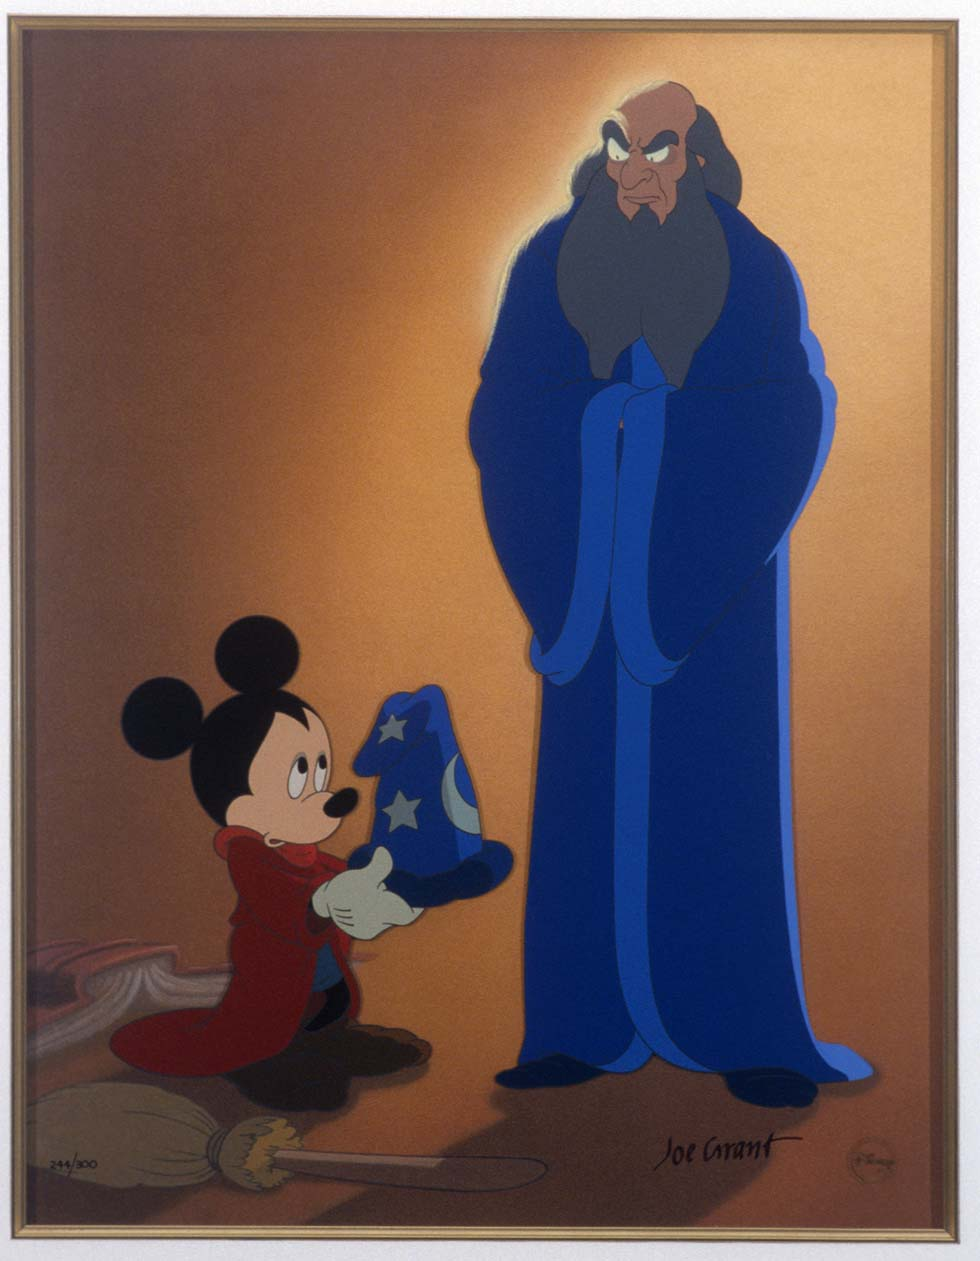
\includegraphics[width=1.0\textwidth]{fantasia}
    \end{figure}
\end{center}
\vspace{\stretch{2}}\null


\cleardoublepage%*******************************************************
% Abstract
%*******************************************************
%\renewcommand{\abstractname}{Abstract}
\pdfbookmark[1]{Resumen}{Resumen}
\begingroup
\let\clearpage\relax
\let\cleardoublepage\relax
\let\cleardoublepage\relax

\chapter*{Resumen}

En esta tesis se describe el diseño e implementación de un codificador JPEG que
utiliza programación genética para buscar una mejor compresión. Para esto se
implementa el algoritmo de codificación JPEG, que luego se transforma en una
función de selección. Se implementan un versión secuencial y una paralela, así
como una implementación para el GPU.

El resultado es un nuevo codificador, que escribe archivos en formato JPEG pero
que puede generar imágenes con mejor calidad y menor tamaño.



\vfill

\endgroup

%%% Local Variables:
%%% mode: latex
%%% ispell-local-dictionary: "espanol"
%%% TeX-engine: xetex
%%% TeX-master: "../Tesis_RGC"
%%% End:

%\cleardoublepage%*******************************************************
% Acknowledgments
%*******************************************************
\pdfbookmark[1]{Agradecimientos}{agradecimientos}

\begin{flushright}{\slshape
        ``In the information age, the barriers just aren't there. \\
        The barriers are self-imposed. If you want to set off and\\
        go develop some grand new thing, you don't need millions \\
        of dollars of capitalization. You need enough pizza and  \\
        Diet Coke to stick in your refrigerator, a cheap PC to   \\
        work on, and the dedication to go through with it.       \\
        We slept on floors.  We waded across rivers."            \\
    %--- \defcitealias{knuth:1974}{Donald E. Knuth}\citetalias{knuth:1974} \citep{knuth:1974}
    --- \textit{John D. Carmack}}
\end{flushright}



\bigskip

\begingroup
\let\clearpage\relax
\let\cleardoublepage\relax
\let\cleardoublepage\relax
\chapter*{Agradecimientos}

Quiero agradecer a mis papás por tolerar la tardanza. A Lore Reynoso, porque me
ayudó a levantarme cuando quería quedarme sentado. A Carolina Barberena, por
ser mi compañera en el último trayecto. A Fabian Giesen, por apuntarme hacia la
dirección correcta.

Muchas gracias a  David Flores, José Galaviz, Gustavo De la Cruz Martínez, Iván
Vladimir Meza y  Elisa Viso.

A Rodrigo González del Cueto, por los litros de café y cientos de horas,
compartiendo el arte de la programación hasta que se nos acababa la voz.


\bigskip


\endgroup

%%% Local Variables:
%%% mode: latex
%%% ispell-local-dictionary: "espanol"
%%% TeX-engine: xetex
%%% TeX-master: "../Tesis_RGC"
%%% End:

\pagestyle{scrheadings}
\cleardoublepage%*******************************************************
% Table of Contents
%*******************************************************
%\phantomsection
\refstepcounter{dummy}
\pdfbookmark[1]{\contentsname}{tableofcontents}
\setcounter{tocdepth}{2} % <-- 2 includes up to subsections in the ToC
\setcounter{secnumdepth}{3} % <-- 3 numbers up to subsubsections
\manualmark
\markboth{\spacedlowsmallcaps{\contentsname}}{\spacedlowsmallcaps{\contentsname}}
\tableofcontents
\automark[section]{chapter}
\renewcommand{\chaptermark}[1]{\markboth{\spacedlowsmallcaps{#1}}{\spacedlowsmallcaps{#1}}}
\renewcommand{\sectionmark}[1]{\markright{\thesection\enspace\spacedlowsmallcaps{#1}}}
%*******************************************************
% List of Figures and of the Tables
%*******************************************************
\clearpage

\begingroup
    \let\clearpage\relax
    \let\cleardoublepage\relax
    \let\cleardoublepage\relax
    %*******************************************************
    % List of Figures
    %*******************************************************
    %\phantomsection
    \refstepcounter{dummy}
    %\addcontentsline{toc}{chapter}{\listfigurename}
    \pdfbookmark[1]{\listfigurename}{lof}
    \listoffigures

    \vspace*{8ex}

    %*******************************************************
    % List of Tables
    %*******************************************************
    % \phantomsection
    % \refstepcounter{dummy}
    % \addcontentsline{toc}{chapter}{\listtablename}
    % \pdfbookmark[1]{\listtablename}{lot}
    % \listoftables

    % \vspace*{8ex}
%   \newpage

    %*******************************************************
    % List of Listings
    %*******************************************************
    % \phantomsection
    % \refstepcounter{dummy}
    %\addcontentsline{toc}{chapter}{\lstlistlistingname}
    % \pdfbookmark[1]{\lstlistlistingname}{lol}
    % \lstlistoflistings

    % \vspace*{8ex}

    %*******************************************************
    % Acronyms
    %*******************************************************
    %\phantomsection
    % \refstepcounter{dummy}
    % \pdfbookmark[1]{Acronyms}{acronyms}
    % \markboth{\spacedlowsmallcaps{Acronyms}}{\spacedlowsmallcaps{Acronyms}}
    % \chapter*{Acrónimos}
    % \begin{acronym}[UML]
    %   \acro{GA}{Algoritmo Genético (Genetic Algorithm)}
    %   \acro{DE}{Evolución Diferencial (Differential Evolution)}
    %   \acro{PSO}{Optimización por Enjambre de Partículas (Particle Swarm Optimization)}
    %   \acro{CUDA}{Arquitectura Unificada de Dispositivos de Cómputo (Compute Unified Device Architecture)}
    %   \acro{OpenCL}{Lenguaje de Computo abierto (Open Computing Language)}
    %   \acro{GPGPU}{Cómputo de Propósito General en Unidades de Procesamiento Gráfico (General-Purpose Computing on Graphics Processing Units)}
    %   \acro{API}{Application Programming Interface}

    %   \acro{UML}{Unified Modeling Language}
    % \end{acronym}
\endgroup

\cleardoublepage

%%% Local Variables:
%%% mode: latex
%%% ispell-local-dictionary: "espanol"
%%% TeX-engine: xetex
%%% TeX-master: "../Tesis_RGC"
%%% End:


% **********
% Mainmatter
% **********

\pagenumbering{arabic}

% \setcounter{page}{90}
% use \cleardoublepage here to avoid problems with pdfbookmark

\cleardoublepage

\pretolerance=10000
\tolerance=2000
\emergencystretch=10pt


% CORREGIR pixel, truco
\chapter{Introducción}\label{ch:introduction}

La \gls{Compresión de Datos} es el acto de transformar la respresentación de la
información con el propósito de reducir su tamaño.

Se le llama \emph{compresión sin pérdida} a la compresión que se hace de manera
que la información representada se mantenga intacta. Por otro lado, la
\emph{compresión con pérdida} es una transformación que reduce el tamaño de la
representación y que permite un grado de pérdida de información.

Un ejemplo de compresión es el uso de la multiplicación para escribir sumas
repetidas de una manera más corta, o de la exponenciación, que comprime de la
misma manera la multiplicación repetida.

$ a + a + a + a + a $ se comprime con $ 5 * a $. Ambas ecuaciones contienen la
misma información, el acto de comprimir reduce el tamaño de la
\emph{representación}, dejando intacto el significado.

La Compresión de Datos es una de las ramas más viejas de las Ciencias de la
Computación. Está sentada sobre fundamentos matemáticos solidificados durante
el mismo periodo en el cual las Ciencias de la Computación se establecían como
un campo legítimo de estudio \cite{cs_the_discipline}.

Es un matrimonio entre teoría y práctica que combina el rigor matemático de las
teorías en las que se basa y el ingenio y la eficacia del implementador.

\section{Motivación}

A principios de la década de 1990, cuando la popularidad de Internet estaba
iniciando su crecimiento exponencial, un comité de matemáticos e ingenieros,
llamado "Joint Photographic Experts Group", o \gls{JPEG} estandarizó un formato de
compresión de imágenes \cite{jpeg-spec}. El formato JPEG, soportando varios
métodos de compresión, fue adaptado rápidamente y hoy en día es soportado por
prácticamente todo programa que tenga que leer imágenes. Imágenes JPEG están
incluidas en millones de páginas web y virtualmente todo navegador lo soporta.

Por su naturaleza, los formatos de datos son esclavos a la inercia. Mientras
nuestro nuevo conocimiento matemático nos da herramientas que podemos utilizar
para crear técnicas más eficientes y compresión de mayor calidad, los datos
viejos siguen estando en sus viejos formatos y migrar puede ser difícil o
imposible. En el caso de compresión con pérdida, migrar datos a nuevos formatos
hace que se pierda parte de la información. Ésta pérdida, en muchos casos, es
un precio demasiado alto que pagar para obtener las ventajas de nuevos y
mejores formatos con compresión de datos.

Como resultado, se puede notar que la adopción de nuevas técnicas de compresión
tiende a ir de la mano con la migración a nuevos medios tecnológicos, e.g. VHS
a DVD. Es poco probable que en el corto o mediano plazo veamos una migración
tecnológica que nos haga cambiar fundamentalmente la manera que guardamos y
compartimos fotografías. JPEG es la técnica de compresión con pérdida es más
utilizada en el mundo y no hay razón para pensar que eso va a cambiar en el
futuro cercano.

Dado que las computadoras son mucho más rápidas de lo que eran en los 90s, y
dada la dificultad de adoptar nuevos formatos de compresión, la motivación de
este trabajo viene de la pregunta:  ¿Qué se puede hacer con el poder de sobra
que tenemos a nuestra disposición?

El resultado este trabajo es una manera de obtener una compresión JPEG de mejor
calidad a la de codificadores convencionales, usando un algoritmo genético.

\section{Objetivo}

La compresión JPEG, que será descrita en el capítulo \ref{ch:jpeg_desc}, tiene
un componente importante para el cual no existe solución óptima. El componente
al que me refiero es un par de matrices cuadradas de tamaño $8\times8$. La
elección de qué matrices elegir para comprimir una imagen determina en gran
parte la calidad y la tasa de compresión.

La especificación JPEG \cite{jpeg-spec} incluye matrices de ejemplo, pero la
elección de qué par de matrices usar está en las manos de cada codificador
JPEG. En la mayoría de los casos, cada implementador deja fijas en su
codificador una lista de pares de matrices que corresponden a diferentes
niveles de calidad. Las matrices se generan \"a ojo\". Sabiendo cómo funciona
el algoritmo, y probando la calidad de la compresión para cada matriz sobre un
conjunto fijo de imágenes que se consideran representativas.

El enfoque de este trabajo es producir un codificador JPEG que encuentre un par
de matrices ideal para la imagen particular que se está decidiendo codificar.
Se implementó un codificador JPEG diseñado desde cero para adaptarse a un
algoritmo genético. La implementación hace uso del paralelismo en CPUs y GPUs.

En los siguientes capítulos, se da una descripción del funcionamiento de la
compresión JPEG y una introducción a los algoritmos genéticos. Después, se da
una descripción de los detalles de la implementación, seguido de un desglose de
los resultados y una sección donde se habla de las conclusiones obtenidas.


  % escrito! editado!
%************************************************
\chapter{Descripción de compresión JPEG con pérdida}\label{ch:jpeg_desc}
%************************************************

\section{Historia y Descripciones Breves de los Fundamentos Matemáticos}

La Teoría de Codificación es una sub-rama de la Teoría de la Información que
marcó el inicio del estudio formal de la compresión de datos. La Teoría de la
Información, nacida en 1948 con la publicación del artículo de Claude E.
Shannon ``A Mathematical Theory of Communication'' \citep{shannon}, gira
alrededor de los conceptos de \emph{densidad de información}, \emph{entropía de
información} y \emph{redundancia de información}.

La Codificación de Entropía son métodos de compresión sin pérdida de
información que no toman en cuenta el contenido. Los dos métodos más populares
actualmente son los Códigos de Huffman y la Codificación Aritmética.

Dos años después de la publicación de Shannon, David Huffman inventó lo que hoy
conocemos como Codificación Huffman \citep{Huffman}. Los Códigos de Huffman son
códigos de prefijos que minimizan la longitud de los códigos individuales. Se
mantienen hasta hoy como la técnica más aprovechada en algoritmos de compresión
sin pérdida.

Después de Huffman, el método más popular para reducir redundancia es la
Codificación Aritmética. Es un método más sofisticado que consigue mejores
resultados. Entre $5\%$ y $10\%$ según el estándar JPEG \citep{JPEGSTD}. La
especificación de la compresión JPEG incluye la capacidad de utilizar
codificación aritmética, pero en la práctica no tiende a ser usada. En
particular, las implementaciones de código abierto no podían usar legalmente
Codificación Aritmética ya que es una técnica altamente patentada
\citep{jpeg_patents}.

En 1974, Nasir Ahmed publicó un artículo describiendo su Transformada de Coseno
Discreta \emph{(DCT)}, por sus siglas en Inglés. La DCT es un caso particular
de la transformada de Fourier, restringida a los números reales.

La compresión JPEG como casi todos la usamos se basa en códigos de Huffman y en
la Transformada de Coseno Discreta.

% ============================================================
\section{Tipos de compresión}
% ============================================================

La compresión de datos puede ser \emph{con pérdida} o \emph{sin pérdida}. Una
compresión sin pérdida es una función biyectiva. El dominio de la función es el
espacio de datos que estamos interesados en comprimir. Los formatos de
compresión sin péridida funcionan identificando información redundante y
removiendo la redundancia, dejando la información intacta. La compresión con
pérdida hace esto también, pero también identifica información ``inecesaria''.
Dependiendo de la agresividad de la compresión, la pérdida de información puede
ser desde imperceptible a inaceptable.

El formato JPEG soporta varios tipos de compresión.

\begin{list}{}{} \item \emph{Baseline}

El tipo \emph{baseline} es el más popular y es el tipo de compresión en el que
se enfoca este trabajo. Por brevedad, a menos de que se especifique lo
contario, cuando el resto de este documento hable de compresión JPEG, estará
hablando del tipo \emph{baseline}. La compresión está basada en la Transformada
de Coseno Discreta para filtrar información innecesaria, y para reducir
redundancia puede utilizar Árboles de Huffman o Codificación Aritmética.

\item \emph{Progresivo}

El tipo \emph{progresivo} es similar a \emph{baseline}, pero se le agregan
propiedades deseables. La imagen se comprime en múltiples pasos, cada uno con
mayor detalle. Con el método \emph{progresivo}, se puede desplegar la imágen
sin que se tenga la totalidad de los datos en memoria.

La utilidad de este método es poder dibujar la imágen mientras se está
descargando de Internet. Cuando se está en un entorno con ancho de banda
limitado, o cuando se descarga una imágen muy grande, es de valor para el
usuario poder ver versiones de la imágen progresivamente más detalladas
mientras se descarga.

\item \emph{Sin pérdida}

La compresión sin pérdida fue agregada a JPEG ``por que tenían que'' y no hubo
un análisis riguroso para su diseño \citep{JPEGSTD}. Aunque la compresión JPEG
sin pérdida no es mala, formatos como PNG son altamente más populares y
efectivos. Mucho software simplemente no soporta JPEG con compresión sin
pérdida.

\item \emph{Compresión Jerárquica}

El modo jerárquico codifica la imágen en varias versiones, cada una a
diferentes resoluciones. Se guarda en una estructura ``piramidal''. La primera
imágen está comprimida a resolución completa, y cada imágen sucesiva se guarda
a la mitad de la resolución de la anterior. Esta pirámide se guarda en memoria
de imágen más pequeña a imágen más grande.

Este método es útil cuando la resolución de la imagen es muy grande, y la
aplicación no necesita o no es capaz de utilizar la imagen en su tamaño
completo.

\end{list}

% ============================================================
\section{Descripción de la Compresión \emph{Baseline} de JPEG}
% ============================================================

El codificador implementado en este trabajo es el \emph{Baseline JPEG}, al que
también se le refiere como \emph{DCT-Based Coding}, traducido aquí como
\emph{Codificación DCT}. Para el resto del documento, a menos que sea
necesario, se usará el término \emph{JPEG} para referirse a lo mismo que
\emph{Baseline JPEG}.

La codificación DCT divide a la imágen en bloques de $8\times8$ píxeles. Cada
bloque de $8\times8$ pasa por una serie de transformaciones y salen
secuencialmente como datos comprimidos.

El primer paso en el \emph{pipeline} es separar los componentes de la imágen.
Las dos maneras más comunes de representar imágenes en computadoras es
\verb+RGB+ o \verb+RGBA+: En ambos formatos, cada píxel ocupa 32 bits de
espacio, divididos en componentes de 8 bits. Cada componente corresponde a un
color o al valor de opacidad, comúnmente denominado \emph{alpha}. \verb+RGB+
corresponde al byte \verb+RRGGBBXX+, con \verb+RR+ representando rojo,
\verb+GG+ representando verde y \verb+BB+ representando azul. Aunque a veces
decimos que \verb+RGB+ es un formato de 24 bits, especificamos el byte
\verb+XX+ por convención, ya que siempre se utilizan 32 bits (4 bytes) para
representar RGB. \verb+RGBA+ es análogo a \verb+RGB+. Le corresponden los 4
bytes \verb+RRGGBBAA+, donde el último byte se usa para el valor \emph{alpha}.

\subsection{Endianness}

Cabe notar que diferentes plataformas tienen diferentes convenciones para
guardar colores en memoria. Windows espera que le mandemos píxeles en órden
\verb+BGRA+, ya que al inspeccionar la memoria se ve en el órden más familiar
de \verb+ARGB+ (Microsoft no ha dicho públicamente por qué reordenaron los
componentes de color pero no el de opacidad).

Este tema toca el concepto de \emph{endianness}, que es el término que usamos
para referirnos al orden de los bytes en una palabra de memoria. En
procesadores modernos, una palabra son 32 bits. 4 bytes, cada uno de 8 bits. La
mayoría de las instrucciones que se ejecutan toman palabras como parámetros, y
cuando nos importan los detalles de bajo nivel entonces debemos de entender la
diferencia entre arquitecturas \emph{little endian} y \emph{big endian}. Una
arquitectura \emph{Little endian} guarda los bytes de una palabra de izquierda
a derecha del menos significativo al más significativo. Es más claro usar el
ejemplo concreto de los colores representados en palabras de 32 bits. Un color
\verb+RGBA+ consiste de 4 bytes y en una máquina little endian se guarda en la
memoria de la computadora como \verb+ABGR+. En una máquina \emph{big endian},
se guarda de la misma manera en que lo escribirmos: \verb+RGBA+. En ambos tipos
de ordenamiento de memoria, su \emph{endianness} afecta sólamente al
ordenamiento de bytes dentro de palábras de máquina. No hay que confundirnos y
pensar que el efecto se extiende más allá de una palabra de 32 bits. Si tenemos
dos palabras \verb+U = abcd+ y \verb+V = efgh+ entonces \verb+UV+ se ve en
memoria como \verb+dcbahgfe+. Los bytes se voltean dentro de las palabras
individuales, pero las palabras siempre van de izquierda a derecha.
Procesadores ARM después de la versión 3 son \emph{bi-endian}; pueden
seleccionar su \emph{endianness} desde software.

En ensamblador con sintaxis de Intel o en el API de Windows, se utiliza
\verb+BYTE+ para denotar 8 bits, \verb+WORD+ para 16 bits, \verb+DWORD+ para 32
bits y \verb+QWORD+ para 64 bits. Esta convención viene de cuando los
procesadores eran de 16 bits, y no cambió ni en la transición a 32 bits en los
90's ni en la transición a 64 bits en los 00's

El codificador JPEG que escribimos asume que la máquina en la que se está
corriendo es \emph{little endian}.


\subsection{La DCT}

La transformada discreta de coseno, \emph{DCT} por sus siglas en Inglés, puede
representar $N$ puntos como una suma con pesos de funciones cosenoidales de
diferentes frecuencias. Es popular en compresión porque las señales que
comprimimos tienden a tener una representación con bajas frecuencias
predominantes. Por ejemplo, es más común una imagen de un cielo azul que ruido
blanco en todos los colores. Una imagen de un cielo azul tiene muy poca
variación, que al aplicar \emph{DCT} resulta en un peso alto para frecuencias
bajas y pesos más cercanos a cero para frecuencias más altas.

En JPEG, se divide la imagen en bloques de $8\times8$ y se utiliza una \emph{DCT} de $8\times8$:
\begin{equation}\label{eq:dct}
F(u, v) = \frac{1}{4} C(u)C(v) \sum_{x=0}^{7}\sum_{y=0}^{7}
f(x,y)*\cos{\frac{(2x+1)u\pi}{16}}\cos{\frac{(2y+1)v\pi}{16}}
\end{equation}
donde \[C(u), C(v) = \begin{cases}
        \frac{1}{\sqrt{2}} & \quad \text{para } u,v = 0\\
        1                  & \quad \text{para } u,v \neq 0\\
\end{cases} \]
\begin{eqnarray*}
    f(u, v) \text{ es un punto del bloque de } 8\times8 \text{ de la imagen }\\
    F(u, v) \text{ es la DCT para el punto } u,v\\
\end{eqnarray*}

De la ecuación \ref{eq:dct} se puede derivar directamente un algoritmo para la
\emph{DCT}:

\label{alg:dct}
\begin{code}[language=C][h]
    float DCT[64];
    for (int v = 0; v < 8; ++v) {
        for (int u = 0; u < 8; ++u) {
            DCT[v*8 + u] = F(u, v);
            // F es la traducción directa de definición DCT
    }
\end{code}


La implementación de JPEG que escribí se llama \verb+tiny_jpeg+
\citep{tiny_jpeg} y contiene dos implementaciones de \emph{DCT}, la que se
muestra arriba, y una más rápida, desarrollada por \citep{ahmed_dct}.

Los algoritmos rápidos para calcular la \emph{DCT} están basados en la
observación de que la ecuación \ref{eq:dct} es lineal, y por lo tanto el
cálculo \emph{DCT} se puede ver como una multiplicación de dos matrices de
$8\times8$. La matriz de la derecha es el bloque con los valores de la imagen y
la matriz de la izquierda es la representación como matriz de la ecuación
\ref{eq:dct}.

\subsection{YUV}\label{sub:yuv}

Para generar los bloques que van a ser procesados por \emph{DCT}, la imagen se separa en tres componentes. JPEG no usa el espacio de color \verb+RGB+, usa \verb+YUV+, también denominado \verb+YCrCb+

\begin{figure}
    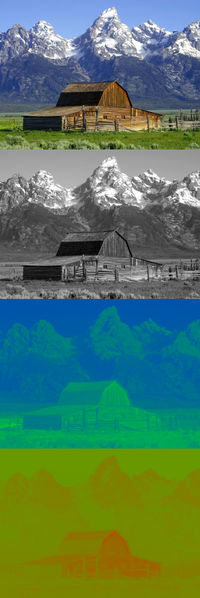
\includegraphics{yuv}
    \caption{Descomposición de una imagen a un canal de Luma y dos de Chroma}
\end{figure}


\verb+Y+ corresponde a Luminancia o Luma


\begin{figure}[hb] % h quiere decir "here". Queremos mostrar la imagen despues de explicar lo que es...
    
\includegraphics{DCT-8x8}
    \caption{Visualización de las funciones para el DCT de 8x8 usado en JPEG. Esquina superior izquierda: menor frecuencia. Inferior derecha: mayor frecuencia.}
\end{figure}

%%% Local Variables:
%%% mode: latex
%%% ispell-local-dictionary: "espanol"
%%% TeX-engine: xelatex
%%% TeX-master: "../tesis"
%
 % <- escrito! editado!
\chapter{Implementación JPEG}\label{ch:implementacion}

Este trabajo empezó como un proyecto motivado por curiosidad para averiguar
cómo funciona JPEG. La idea de usar el GPU salió de notar que el algoritmo
separa a la imagen en bloques que parecían ser independientes. En realidad no
lo son, pero como se verá mas adelante, se encontró una manera de hacer un
codificador paralelo. El progreso culminó en lo que se describe en este
trabajo. El proyecto final se le llamó \emph{gp\_encoder} y su código está en
github \cite{gp_encoder}.

El codificador JPEG fue lanzado al dominio público en \emph{ Github } bajo el
nombre de TinyJPEG \cite{tiny_jpeg}.

En este capítulo se describen los detalles de ambos proyectos.

\section {Términos} Se usan los términos \emph{\gls{depurar}} y
\emph{\gls{profiling}}. Depurar, en computación, se refiere al proceso de
encontrar y arreglar defectos de código. \emph{profiling} es el proceso de
encontrar los puntos en los que un programa puede ser modificado para mejorar
el desempeño.

\emph{General Purpose GPU}, o \emph{\gls{GPGPU}} es el término usado para la
práctica de programar GPU directamente, a diferencia del uso original, donde
el GPU era un acelerador controlado por una biblioteca de gráficas como OpenGL
o DirectX.

% ============================================================
\section{Tecnologías}
% ============================================================

La elección de lenguaje para TinyJPEG fue C. C99 para ser específico
\cite{c99}. TinyJPEG fue lanzado con el objetivo de ser una biblioteca
reutilizable, y ha encontrado cierto grado de éxito. Un planetario en París usa
TinyJPEG para capturar vídeo de sus simulaciones.

C es un lenguaje ideal para escribir cosas como codificadores. El lenguaje
permite mantener el nivel bajo de abstracción que se necesita y las
herramientas de \emph{debugging} son mejores para C y C++ que para casi
cualquier otro lenguaje.

Se escogió OpenCL para la implementación de GPGPU. OpenCL es un estándar abierto
para GPGPU y está soportado por Intel, Nvidia y AMD. La máquina en la que se
implementó este trabajo tiene una tarjeta Nvidia. Nvidia tiene su propio
lenguaje para GPGPU, llamado CUDA, que tiene mejor soporte para debugging y
profiling que OpenCL para sus tarjetas de video. Sin embargo, las herramientas
siguen siendo primitivas comparadas con lo que se tiene en el CPU. En cualquier
caso, uno termina haciendo hipótesis, experimentos y mediciones para optimizar la
solución, aun teniendo herramientas sofisticadas. Se escogió OpenCL porque los
méritos relativos de facilidad de desarrollo de CUDA no le ganan al soporte
multi-plataforma y al valor de apoyar estándares abiertos de OpenCL.

% ============================================================
\section{Arquitectura}
% ============================================================

TinyJPEG es minimalista. Consiste de un archivo de alrededor 1000 líneas. Está
escrito en el estilo popularizado por Sean Barrett \footnote{Sean Barrett es un
programador famoso por escribir el motor de rendering del juego Thief y de sus
bibliotecas de código libre \emph{stb} para facilitar el desarollo de
aplicaciones multimedia.} de escribir un solo archivo \verb+.h+ con la
siguiente estructura:

\label{alg:stb}
\begin{code}[language=C][h]
    // Principio del archivo
    #pragma once

    // Definición de la interfaz.
    tje_encode_to_file(...);

    #ifdef TJE_IMPLEMENTATION

    // La implementación completa va aquí.
\end{code}

De esta manera, uno puede incluir \verb+#include <tiny_jpeg.h>+ como cualquier
encabezado de C, pero en uno de los archivos del proyecto, para definir la
implementación completa, se hace lo siguiente.

\label{alg:stb_impl}
\begin{code}[language=C][h]
    #define TJE_IMPLEMENTATION
    #include <tiny_jpeg.h>
\end{code}

El propósito de esta técnica es facilitar la distribución de bibliotecas en un
lenguaje que no cuenta con un sistema de distribución digital, o siquiera un
sistema de módulos.

Se exponen dos funciones como interfaz pública:

\begin{code}[language=C][h]
tje_encode_to_file(...)
tje_encode_to_file_at_quality(...)
\end{code}

La primera comprime con la tabla unitaria y la segunda ofrece tres posibles
niveles de calidad: ``alto", ``mediano", y ``bajo". Todos correspondientes
únicamente al uso de tres tablas de cuantificación.

Ambas funciones son envolturas sobre la función principal interna, que funciona
de la siguiente manera:

Se prepara una estructura estática para hacer compresión de Huffman y se
pre-procesa la tabla según el algoritmo DCT descrito en \ref{sec:DCT}. A esto
le llamamos el \emph{paso inicial}.  Cuando terminamos el \emph{paso inicial},
determinamos el número de bloques que van a ser procesados. JPEG debe poder
funcionar con imágenes cuyos tamaños verticales y horizontales no sean múltiplos
de 8. Para esto la especificación sólo nos pide como codificador redondear al
siguiente múltiplo de 8. Al decodificador le pide ignorar los datos adicionales. Para
evitar \gls{artefactos}, como convención se repite en el bloque el color del
último píxel de la imagen para cada columna adicional y para cada renglón adicional. Si
$w$ es el ancho de la imagen y $h$ es el alto, y ninguno de los dos es múltiplo
de 8, entonces el número de bloques es $n = (w + (8 - w \mod 8)) * (h + (8 - h
\mod 8))$. Cuando $w$ o $h$ es múltiplo de ocho, entonces se sustituye el
término en la multiplicación por solamente $w$ o $h$ respectivamente. Por
ejemplo, si $w \mod 8 = 0$ entonces $n = w * (h + (8 - h \mod 8))$

Cada bloque se separa en tres bloques \verb+Y+, \verb+U+, \verb+V+, a los que
se les aplica la función \verb+encode_MCU()+.

La función \verb+encode_MCU()+ se llama así por el acrónimo \emph{\gls{MCU}},
\emph{Minimum Coded Unit}. JPEG puede especificar un factor para describir los
bloques \verb+U+ y \verb+V+ con menos resolución, por nuestra relativa falta de
sensibilidad a la crominancia contra la luminancia, pero TinyJPEG no utiliza
esto. Otra posibilidad es usar diferentes tablas de codificación para
lumninancia y crominancia. TinyJPEG sí utiliza esto, escogiendo tablas con
mayor compresión para los bloques de crominancia.

Se usa un par de iteraciones para extraer los bloques, y cada bloque se pasa como
parámetro a la función \verb+encode_MCU+. En pseudo-código:

\begin{code}[language=C][h]
    for ( int y = 0; y < height; y += 8 ) {
        for ( int x = 0; x < width; x += 8 ) {
            for ( int off_y = 0; off_y < 8; ++off_y ) {
                for ( int off_x = 0; off_x < 8; ++off_x ) {
                    int block_index = (off_y * 8 + off_x);
                    // ... llenar bloque
                }
            }
            encode_MCU(bloque);
        }
    }
\end{code}

\subsection{DummyJPEG} \label{sub:dummy}

A primera vista, el algoritmo JPEG se ve ``embarazosamente paralelo". Una
motivación para este trabajo fue la observación de que el algoritmo trabaja
dividiendo la imágenes en cuadros de $8\times8$ y el hecho de que los GPU
actuales trabajan con instrucciones vectoriales de 32 elementos. Actualmente,
cuando se hace \gls{GPGPU}, se considera buena práctica que el tamaño de las
unidades de trabajo sean un múltiplo de la longitud de las instrucciones de la
arquitectura. Por esto, los bloques de 64 elementos se prestan a ser procesados
por GPU actuales.

Desafortunadamente, el algoritmo JPEG no es paralelo. Aplicar codificación
delta al coeficiente DC introduce una dependencia de datos entre cada bloque de
\verb+Y+, \verb+U+ y \verb+V+ respectivamente. Para cada componente, cualquier
bloque después del primero depende del anterior para poder computar la
diferencia entre su coeficiente DC  y el de su antecesor.

Sin embargo, aunque JPEG es inherentemente secuencial para cada componente,
está muy cerca de ser paralelo. Si el \emph{Joint Photographic Experts Group}
no hubiera decidido tratar de manera diferente a los \gls{coeficientes AC} y DC, el
algoritmo sería completamente paralelo.

Se quiere darle la vuelta al problema, y la manera en que se hace es creando
un ``Dummy JPEG": Un algoritmo que es \emph{casi} JPEG, pero que no es correcto.

La implementación de DummyJPEG empieza como un clon directo de TinyJPEG. Lo
primero que se hace es cambiar las función que escribe a disco por una función
que va contando el número de bits. De esta manera, al aplicar el algoritmo no
se tiene una imagen, pero se tiene un reporte del tamaño de la imagen que
se hubiera generado.

También se cambia el algoritmo para aplicar la Transformada Inversa de Coseno
justo después de aplicar la DCT al bloque, para poder compararlos y calcular el
error.

Entonces, si el algoritmo original para cada bloque en TinyJPEG es:

\begin{code}
    x = aplicar_dct(bloque);
    codificar(x)
\end{code}

El algoritmo para cada bloque en DummyJPEG se convierte en esto:

\begin{code}
    x = aplicar_dct(bloque)
    reportar_tamaño(x)
    y = aplicar_idct(x)
    reportar_error(bloque, y)
\end{code}

En donde \verb+reportar_error+ es una suma de la diferencia absoluta entre cada
pixel del bloque original y del bloque reconstruido.

La manera en que se vuelve paralelo a DummyJPEG es simplemente no codificar al
coeficiente DC. Esto introduce un error en el tamaño reportado pero no afecta
al error reportado. El error que se introduce viene de que se cuentan los bits de
la representación de los 63 \gls{coeficientes AC}, pero no se cuentan los bits del
\gls{coeficiente DC}. En las imágenes de prueba que se usaron para este trabajo, el
tamaño reportado es menor que el tamaño real entre un 10\% y 20\%.

La pregunta que se hace es: ¿El error en el reporte de tamaño es significativo?

La presión que se pone en la evolución es hacia imágenes que son
indistinguibles de la original. Como el valor de cuantificación del primer
coeficiente afecta de manera importante la calidad de imagen comprimida, las
tablas de la población rápidamente convergen a tener el primer valor de
cuantificación igual a 1. Esto quiere decir que para casi cualquier conjunto de
tablas que vayamos a comparar, su coeficiente DC es igual. Por lo tanto,
siempre se introduce el mismo error en el reporte de los tamaños de las
imágenes resultantes. Esto nos permite despreocuparnos de no tomar en cuenta el
primer coeficiente.

Otra cosa que se hace es \emph{solo calcular bloques de luminancia}, ya que los
bloques de crominancia usualmente usan una tabla secundaria y el propósito es
evolucionar una sola tabla. Podemos deshacernos de $66\%$ del trabajo si
descartamos los dos componentes de crominancia. Más tarde, cuando se finalice
la evolución, podemos usar la misma tabla para los tres componentes o bajar la
calidad de la tabla para los componentes de crominancia, multiplicando cada
elemento por alguna constante.

Ya que se tiene un algoritmo que es \emph{casi JPEG}, pero paralelo, se sigue
con la tarea de cambiar la arquitectura del programa para paralelizarlo en el
CPU. La razón por la que se implementa el paralelismo en el CPU antes de
hacerlo en el GPU es principalmente la velocidad de desarrollo. La versión
paralela en el CPU se hace pensando en el diseño final para el GPU.  El
código se moldea para que el flujo de ejecución en el CPU sea muy similar a la
manera en que trabaja el GPU, intentando llegar al punto en que la
implementación en el GPU se reduzca a un \emph{copy paste}, pero que el esfuerzo
que se aplique a la implementación del GPU sea solamente un trabajo de
optimización de bajo nivel.

\section{Introducción a GPGPU} \label{sec:gpgpu}

Las arquitecturas de GPU, en el momento que se escribe esto, trabajan con
instrucciones SIMT (\emph{Single Instruction, Multiple Threads}).

Supercomputadoras vectoriales como la \emph{Cray} se introdujeron en la década
de 1970 pero gradualmente perdieron popularidad, mientras computadoras con
microprocesadores x86 bajaron de precio. Las computadoras de escritorio serían
completamente escalares hasta el final de los 90, y las súper-computadoras
seguirían siendo por un tiempo grupos de procesadores x86.

En 1998 AMD introdujo instrucciones vectoriales con su tecnología \emph{3D
Now}, seguido por Intel en 1999 cuando introdujo SSE (Streaming SIMD
extensions). Ambas tecnologías son extensiones al conjunto de instrucciones x86
que introducen cómputo vectorial. Unos años más tarde se empezarían a
popularizar los procesadores \emph{multi-core}. Ambos desarrollos, que
introducen cómputo paralelo a los procesadores para consumidor, son el resultado
de la desaceleración de la velocidad escalar y una demanda constante de mayor desempeño.

Otra respuesta a esta demanda para mayor desempeño nació en los noventas: Los
aceleradores gráficos o GPU, tarjetas que se dedican a rasterizar triángulos
rápidamente para aplicaciones multimedia, principalmente videojuegos.

Aunque al principio los GPU estaban diseñados alrededor de  las API como OpenGL y
DirectX, con funcionalidad fija, poco a poco fueron adquiriendo la habilidad de
ser programables. Primero con \emph{shaders}, que permitieron meter código en
un par de partes clave del proceso de rasterización, y más tarde con OpenCL y
CUDA, que permiten escribir programas para el GPU en un dialecto de C.

El modelo de ejecución de OpenCL corresponde directamente a las arquitecturas
GPU actuales. Para describir su funcionamiento, en este documento se usa la
terminología de OpenCL y AMD. Nvidia tiene términos diferentes para los mismos
conceptos, la tabla \ref{fig:equiv} describe las equivalencias.

Esta descripción se enfoca en la arquitectura Kepler de Nvidia y cómo le
corresponden los conceptos de OpenCL.

Un programa OpenCL opera con \emph{work items}. Un work item puede pensarse
como una \emph{``fibra"} en un \emph{``cable"} que ejecuta instrucciones
vectoriales. En la arquitecturas modernas de Nvidia, la longitud de los
vectores es de 32 elementos. Es decir, cada cable tiene 32 fibras.

A estos \emph{``cables"} se les denomina \emph{wavefronts}.

La tarjeta de video tiene un calendarizador implementado en hardware que
trabaja con granularidad de \emph{wavefronts} individuales. Los \emph{work
items} corren \emph{kernels}, que son funciones escritas en el
dialecto de C de OpenCL para ser ejecutadas en el GPU. Un kernel de OpenCL se
ve como código en C, pero hay que imaginarse que en lugar de un sólo apuntador
de instrucciones avanzando secuencialmente, se está lidiando con 32 apuntadores
de instrucciones (las fibras del cable en la analogía que se usa). Este es un
paradigma diferente. Por ejemplo, los saltos dinámicos se convierten en algo
caro, ya que mientras un subconjunto de los 32 apuntadores de instrucciones
procesa un camino de ejecución, el resto debe esperar. Un salto que se toma el
50\% del tiempo es causa un \emph{slowdown} de 2x.

Un \emph{work item} es parte de un \emph{work group}. El tamaño del \emph{work
group} es decisión del programador, puede ser de 1, 2 o 3 dimensiones y su
tamaño puede variar, aunque es buena práctica escoger un múltiplo del tamaño de
los wavefronts (32 en Kepler y Maxwell). Hay que encontrar el tamaño apropiado
para los \emph{work groups} para minimizar contención de memoria y maximizar el
rendimiento (se usa la palabra rendimiento como traducción directa de de
\emph{throughput}). Los GPU están diseñados para sacrificar latencia por
rendimiento.

Nótese que el concepto de \emph{work group} es una abstracción que se provee
para facilitar la programación en OpenCL. Crear work groups de cierto tamaño y
dimensiones ayuda a visualizar problemas. Sin embargo, es importante tener
siempre en cuenta que un work group siempre es ejecutado por un wavefront.

Cada generación de GPU tiene diferentes características de desempeño. Es útil
usar referencias oficiales \cite{maxwell-tuning}, pero los recursos gratis,
como GPU Tech Conf (GTC) \cite{gtc}, una conferencia anual sobre GPU, son una
buena fuente de información para aprender a obtener el mayor desempeño posible
de las arquitecturas actuales.

En la microarquitectura del GPU, los \emph{wavefronts} son ejecutados en
procesadores vectoriales llamados \emph{Processing Elements}. Cada Processing
Element tiene un número limitado de registros y puede ejecutar un wavefront a la vez.

Cada Processing Element es miembro de un \emph{Compute Unit}, que tiene un caché L1.

El GPU contiene un número de Compute Units, quienes comparten un caché L2 y una
memoria global. En el ejemplo en la figura \ref{fig:kepler1} es un GPU con 15
Compute Units.

Desde el punto de vista del modelo OpenCL solo existe la memoria local y
memoria global. En la práctica, la memoria local corresponde a los registros
del Processing Element y al cache L1. La memoria global corresponde a la
memoria global del GPU, pero la microarquitectura puede encargarse de ``subir''
y ``bajar''  accesos de memoria global por la jerarquía de memoria física.

Durante la ejecución de un kernel. A diferencia de los CPU, no hay garantía de
coherencia cuando se escribe a memoria. OpenCL provee mecanismos de
sincronización de memoria para cuando es absolutamente necesario, pero en la
práctica resultan en un golpe fuerte al desempeño.

La arquitectura de los GPU está diseñada para lidiar con problemas de
contención de memoria. Cuando algún work item dentro de un wavefront está
esperando a que se efectúe una operación de memoria, o está esperando a otro
miembro del wavefront a causa de un salto condicional, el calendarizador hace
que el \emph{compute unit} ejecute otro wavefront que esté listo para ser
ejecutado. Esto ocurre muy rápidamente, no hay un costo alto de cambio de
contexto como al que estamos acostumbrados con threads en sistemas operativos.

Las imágenes \ref{fig:kepler1} y \ref{fig:kepler2}, tomadas de la plática de
Nvidia ``Inside Kepler" \cite{kepler-slides}, ayudan a visualizar cómo
corresponde el modelo OpenCL a una arquitectura GPU. En el caso de Kepler,
podemos ver un SMX como un Compute Unit, y cada Cuda Core como un Processing
Element.

\begin{figure}[h]
    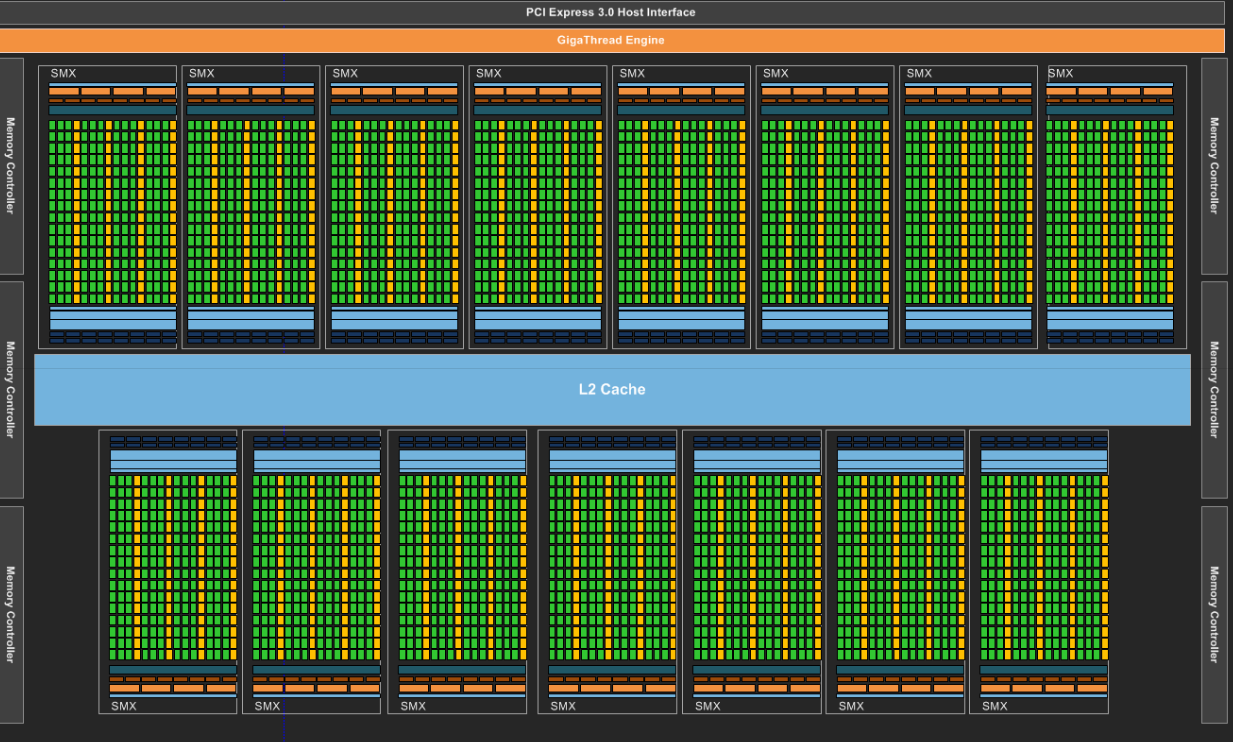
\includegraphics[width=1.0\textwidth]{kepler_1}
    \caption{Compute Units en Nvidia Kepler}
    \label{fig:kepler1}
\end{figure}

\begin{figure}[h]
    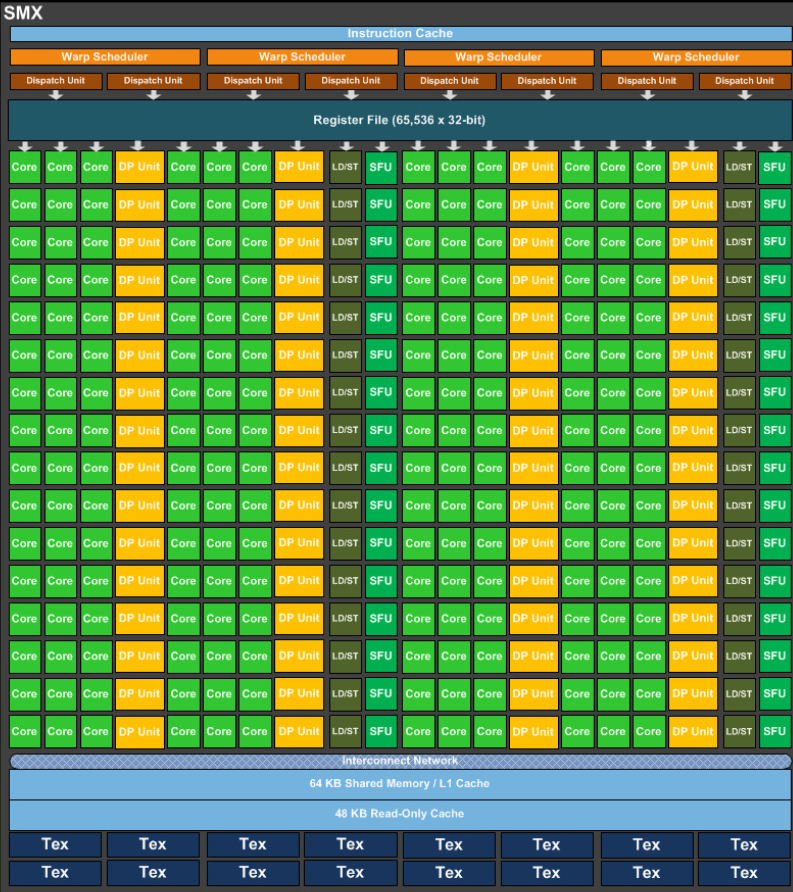
\includegraphics[width=1.0\textwidth]{kepler_2}
    \caption{Processing Elements Dentro de un Compute Unit}
    \label{fig:kepler2}
\end{figure}

\begin{figure}[ht]
    
\includegraphics[width=4.5625in]{fputc}
    \caption{TinyJPEG: 48\%. fputc: 4.8\%}
\end{figure}

El kernel para nuestra función de selección va a hacer el trabajo de la función
\verb+encode_MCU+, que se encarga de tomar bloques de $8\times8$, codificarlos
y reportar el tamaño, y luego decodificarlos y reportar el error.

El kernel de DummyJPEG está diseñado para que cada work item se encargue de un
bloque. Esto quiere decir que cada work group puede estar procesando bloques
completamente distintos. Esto se hace porque cada bloque puede tener un número
arbitrario de ceros una vez que se ha aplicado la \gls{DCT} y se ha aplicado la
cuantificación. Si organizáramos el trabajo de manera que cada workgroup trabaje
con un solo bloque, cada wavefront pasaría la mayor parte del tiempo esperando saltos
condicionales. El problema de los saltos condicionales se discute más adelante
en la sección \ref{sec:microopt}.

\begin {figure}
    \begin{tabular}{ | l | r | }
    \hline
    OpenCL             & Nvidia y CUDA \\
    \hline
    Work Item          & Thread \\
    Work Group         & Thread block \\
    Processing Element & CUDA Core \\
    Compute Unit       & Streaming Multiprocessor (SMX) \\
    \hline
    \end{tabular}
    \label{fig:equiv}
\end{figure}

\section{Implementación paralela en CPU}

Para describir la versión paralela de \verb+encode_MCU+, primero hay que listar
los parámetros que toma la función secuencial, que es llamada una vez por cada
bloque.

\begin{enumerate}
    \item \verb+mcu+, el \emph{minimum coded unit}. Es decir, el bloque
        $8\times8$
    \item \verb+qt+, la tabla de cuantificación (puede ser de luminancia o
        crominancia)
    \item \verb+huffman+, apuntadores a las tablas de huffman para coeficientes
        DC y AC.
\end{enumerate}

Para todos los bloques, los elementos 2 y 3 se mantienen invariantes. Lo que se
hace es cambiar la función para que opere sobre un arreglo de bloques de
entrada y que escriba a un arreglo de salida.

Si hay $n$ bloques en la imagen, DummyJPEG procesa $n$ bloques a la vez y
escribe a un arreglo de $n$ resultados. Un resultado es una tupla $(b, e)$
donde $b$ es el número de bits que el bloque consume después de ser codificado
y $e$ es la suma de las diferencias absolutas pixel-por-pixel entre el bloque
original y el bloque descomprimido.

Como se quiere que la implementación paralela en el CPU sea tan similar al
kernel OpenCL final como sea posible, agregamos un nuevo parametro,
\verb+block_i+. Como su nombre sugiere, es un índice que indica el bloque al
que la función tiene que acceder y el índice a donde tiene que escribir su
resultado.

El algoritmo paralelo trabaja en un patrón \emph{map-reduce}. No en el sentido
de utilizar un cluster de computadoras para cómputo paralelo, si no en los
conceptos de programación funcional que motivaron el título. Es un algoritmo
estilo \emph{map-reduce} porque la mayor parte del cómputo se realiza en
paralelo sobre elementos de un arreglo (correspondiente a la función map) y
cuando el proceso paralelo termina, se realiza una recolección secuencial para
obtener  el resultado final (el equivalente a la función \emph{reduce}). Al implementar una
versión paralela de \verb+encode_MCU+, ya se tiene la función map. Entonces la
función \emph{reduce} consiste de:

\label{alg:mcu_paralelo}
\begin{code}
    B_total = 0;
    E_total = 0;
    Para todo resultado (B, E):
       B_total += B;
       E_total += E;
    Terminar el algoritmo, regresando (B_total, E_total).
\end{code}

La tupla que regresa DummyJPEG son los parámetros $e(T)$ y $s(T)$ de la función de selección
\ref{eq:fitness}.

En el cpu, la parte \emph{map} del algoritmo se ve así:

\begin{code}[language=C][h]
    // Versión de un solo thread.
    for (int i = 0; i < num_bloques; ++i) {
        encode_MCU(i, mcus, qt, huffman);
    }
\end{code}

Para múltiples threads, se utilizan threads trabajadores que consumen unidades
de trabajo. Como se muestra con el siguiente pseudo código:

\begin{code}[language=C][h]
    bool loop = true;
    while ( loop ) {
        // Pseudo-código para el thread trabajador

        int block_i = -1;

        // Sección crítica
        lock();
        if ( bloques_consumidos < num_bloques ) {
            int block_i = bloques_consumidos++;
        } else {
            loop = false;
        }
        unlock();

        if ( block_i >= 0 ) {
            encode_MCU(block_i, mcus, qt, huffman);
        }
    }
\end{code}

El producir trabajo se reduce a esto:

\begin{code}[language=C][h]
    // Apuntar al lugar correcto una variable que los
    // trabajadores puedan accesar.
    g_MCUs = mcus;

    // Cada trabajador lo incrementa atómicamente.
    bloques_consumidos = 0;

    lanzar_trabajadores();
\end{code}

\section{Paralelización en GPU}

Una vez que la implementación paralela funciona en el CPU, es hora de hacer la
implementación OpenCL de DummyJPEG. Como OpenCL usa un dialecto de C, se puede
reutilizar código entre las dos implementaciones de DummyJPEG. Se usa el mismo
código para la DCT y la IDCT. El kernel no es exactamente un \emph{copy paste},
pero la implementación es bastante parecida. Los únicos cambios que se realizan
son en la firma de la función, que tiene sintaxis de OpenCL para especificar
que la función es un kernel y para definir si los parámetros están en memoria
global o en memoria constante.

En la sección \ref{sec:gpgpu} no se habló de memoria constante porque es
operacionalmente igual a la memoria global. La ventaja de usar memoria
constante es que es más fácil de optimizar para el driver, por la garantía de no-escritura.

La firma del kernel \verb+encode_MCU+ es:

\begin{code}[language=C][h]
__kernel void
cl_encode_and_write_MCU(
    /*0*/__global DJEBlock* mcu_array,
    /*1*/__global uint* bitcount_array,
    /*2*/__global ulong* out_mse,
    /*3*/__global float* qt,
    /*4*/__constant uchar* huff_ac_len)
\end{code}

Como se discutió, se convierte \verb+encode_MCU+ en un kernel y se utiliza una
variable global de OpenCL para determinar el bloque con el que se está
trabajando.

\begin{code}[language=C][h]
    // Obtener el indice de bloque en OpenCL
    int block_i = (int)get_global_id(0);
\end{code}
{p
La gran mayoría del esfuerzo en implementar la versión paralela en GPU es en
hacer la inicialización necesaria para que OpenCL establezca una línea de
comunicación entre el CPU y el GPU. Para referencia, ver los archivos
\verb+gpu.c+ y \verb+gpu.h+ en el código fuente del proyecto. Entre las cosas
que se necesitan hacer están: Encontrar un dispositivo OpenCL (el GPU,
idealmente, aunque OpenCL está diseñado para ser una API genérica); Crear un
contexto OpenCL, la estructura que mantiene el estado de la API; Y finalmente
compilar el kernel.

Durante la ejecución, se debe hacer el manejo de memoria de GPU. Todos los
parámetros del kernel son apuntadores a localidades de memoria global en el GPU
que se crean con OpenCL como objetos llamados \emph{OpenCL buffers}. Algunos de
ellos, como las tablas de Huffman, no cambian durante el programa. Otros, como
la tabla de cuantificación, cambia con cada llamada al kernel. Se tiene que
asegurar no tener \emph{memory leaks} y de no borrar buffers mientras están
siendo usados.

Aunque no es una API ideal, el trabajo de inicialización y de manejo de memoria
es relativamente fácil si uno sigue al pie de la letra la especificación de
OpenCL 1.1 \cite{opencl-spec}

Afortunadamente, la estrategia de hacer la implementación paralela en el CPU,
pensando en GPU, para después migrar el trabajo al GPU fue exitosa. La
implementación paralela en GPU requirió de sólo el mínimo esfuerzo necesario,
dejando tiempo para hacer las micro-optimizaciones que se describen en la
sección \ref{sec:microopt}.

El algoritmo funciona correctamente en tres modalidades: Un thread, Múltiples
threads, y GPU. Para un conjunto de imágenes de prueba, la tabla
\ref{fig:perf_table_orig} muestra el tiempo en segundos que cada modalidad toma
para realizar la evolución de la tabla de cuantificación y escribir el JPEG
resultante.

\begin{figure}[h]
    \begin{tabular}{ |l c c c c r| }
        \hline
        Nombre &  Un Thread & Múltiples Threads & GPU & Speedup MT & Speedup GPU \\
        \hline
        Diego & 10.796s & 5.210s & 1.391s  & 2.072X & 7.76X \\
        Ghost & 13.706s & 6.607s & 1.760s  & 2.257X & 7.78X \\
        Klay & 40.526s & 22.279s & 4.785s  & 1.819X & 8.46X \\%, 4.65
        Plutón & 558.83s & 204.120s & 13.940s & 2.73X & 40.08X \\ % 14.64
        \hline
    \end{tabular}
    \caption{Tabla de desempeño para gp\_encoder}
    \label{fig:perf_table_orig}
\end{figure}

Más adelante se describen las características de las cuatro imágenes de prueba
\ref{sec:testset}. Cabe notar que aunque la implementación GPU es siempre más
rápida, en el caso de la imagen ``Plutón", que mide 192MB, el beneficio del GPU
crece por un factor de alrededor de 5X comparándolo con la modalidad CPU con un
thread. Es posible que la razón sea que el trabajo a realizar crece
proporcionalmente con el tamaño de la imagen, y los GPU están diseñados para
rendimiento, no latencia. Se puede especular sobre la razón verdadera. Puede
que el hecho de que haya más wavefronts en vuelo permita que los Compute Units
tengan una mayor utilización, mientras que el menor número de wavefronts para
las imágenes más pequeñas cause problemas de utilización cuando muchos
wavefronts están ejecutando código con saltos condicionales, como el proceso en
JPEG en el que se busca el útlimo elemento del bloque que no es cero. Otra
explicación sería que con imágenes grandes, el calendarizador puede hacer un
mejor trabajo dándole la vuelta a problemas de contención de memoria.


% ============================================================
\section{Algoritmo DCT} \label{sec:DCT}
% ============================================================

A partir de la ecuacion \ref{eq:dct} se puede derivar directamente un algoritmo
simple para la \emph{DCT}:

\begin{figure}
    \begin{code}[language=C][h]
        float DCT[64];
        for (int v = 0; v < 8; ++v) {
            for (int u = 0; u < 8; ++u) {
                DCT[v*8 + u] = F(u, v);
                // F es la traducción directa de definición DCT
            }
        }
    \end{code}
    \caption{Algoritmo DCT derivado directamente}
    \label{alg:dct}
\end{figure}

\verb+tiny_jpeg+ contiene dos implementaciones de \emph{DCT}, la que se deriva
directamente de la ecuación \ref{eq:dct} y que muestra en la tabla \ref{alg:dct}.

El algoritmo \ref{alg:dct} no es práctico para un codificador JPEG y mucho
menos para este proyecto, que ejecuta el algoritmo JPEG cientos de veces para
una sola imagen. Existen métodos para calcular la DCT (y su inversa, la IDCT)
rápidamente. La discusión presentada aquí sobre el desarrollo de algoritmos
rápidos DCT es análoga para la inversa, ya que las ecuaciones son muy similares
(\ref{eq:dct}, \ref{eq:idct}).

Este proyecto usa el algoritmo \gls{DCT} usado en proyectos como ffmpeg y la
implementación de referencia de JPEG. Fue originalmente desarrollado por
\cite{ahmed_dct}.

El algoritmo está basado en la observación de que la ecuación \ref{eq:dct} es
lineal, y por lo tanto el cálculo \emph{DCT} se puede expresar como $F(X) =
A^{T}XA$ Donde $X$ es un bloque de $8\times8$ y A es la matriz:

\begin{equation}
    \label{eq:dct-matrix}
    \begin{bmatrix}
        \frac{\sqrt{2}}{2} & \frac{\sqrt{2}}{2} & \frac{\sqrt{2}}{2} & \frac{\sqrt{2}}{2} & \frac{\sqrt{2}}{2} & \frac{\sqrt{2}}{2} & \frac{\sqrt{2}}{2} & \frac{\sqrt{2}}{2} \\
        cos\frac{\pi}{16} & cos\frac{3\pi}{16}& cos\frac{5\pi}{16}& cos\frac{7\pi}{16}& cos\frac{9\pi}{16}& cos\frac{11\pi}{16}& cos\frac{13\pi}{16}& cos\frac{15\pi}{16} \\
        cos\frac{2\pi}{16} & cos\frac{6\pi}{16}& cos\frac{10\pi}{16}& cos\frac{14\pi}{16}& cos\frac{18\pi}{16}& cos\frac{22\pi}{16}& cos\frac{26\pi}{16}& cos\frac{30\pi}{16} \\
        cos\frac{3\pi}{16} & cos\frac{9\pi}{16}& cos\frac{15\pi}{16}& cos\frac{21\pi}{16}& cos\frac{27\pi}{16}& cos\frac{33\pi}{16}& cos\frac{39\pi}{16}& cos\frac{45\pi}{16} \\
        cos\frac{4\pi}{16} & cos\frac{12\pi}{16}& cos\frac{20\pi}{16}& cos\frac{28\pi}{16}& cos\frac{36\pi}{16}& cos\frac{44\pi}{16}& cos\frac{52\pi}{16}& cos\frac{60\pi}{16} \\
        cos\frac{5\pi}{16} & cos\frac{15\pi}{16}& cos\frac{25\pi}{16}& cos\frac{35\pi}{16}& cos\frac{45\pi}{16}& cos\frac{55\pi}{16}& cos\frac{65\pi}{16}& cos\frac{75\pi}{16} \\
        cos\frac{6\pi}{16} & cos\frac{18\pi}{16}& cos\frac{30\pi}{16}& cos\frac{42\pi}{16}& cos\frac{54\pi}{16}& cos\frac{66\pi}{16}& cos\frac{78\pi}{16}& cos\frac{90\pi}{16} \\
        cos\frac{7\pi}{16} & cos\frac{21\pi}{16}& cos\frac{35\pi}{16}& cos\frac{49\pi}{16}& cos\frac{63\pi}{16}& cos\frac{77\pi}{16}& cos\frac{91\pi}{16}& cos\frac{105\pi}{16}
    \end{bmatrix}
\end{equation}

Esta matriz tiene alta redundancia. Por ejemplo, el cuarto elemento del segundo renglón es $cos\frac{7\pi}{16} \approx 0.19509$. Este va a ser el mismo valor para todos los elementos que sean $cos\frac{n\pi}{16}$ con $n \mod 16 = 7$. Dígase $\frac{25\pi}{16}$, y $\frac{39\pi}{16}$.

Para simplificar la representación se usa el módulo 16 como se acaba de mostrar junto con dos técnicas más: la periodicidad del coseno: $\Big( cos(x) = cos(x + 2\pi) \Big)$ y la propiedad de que es una función par: $\Big( cos(-x) = -cos(x) \Big)$.

Se termina con una matriz cuyos elementos tienen 7 posibles valores y sus negativos:

\begin{equation}
    \label{eq:dct-matrix-simple}
    \sqrt{2}/2
    \begin{bmatrix}
        1 & 1 & 1 & 1 & 1 & 1 & 1 & 1  \\
        a & c & d & f & -f & -d & -c & -a \\
        b & e & -e & -b & -b & -e & e & b \\
        c & -f & -a & -d & d & a & f & -c \\
        1 & -1 & -1 & 1 & 1 & -1 & -1 & 1\\
        d & -a & f & c & -c & -f & a & -d \\
        e & -b & b & -e & -e & b & -b & e \\
        f & -d & c & -a & a & -c & d & -f
    \end{bmatrix}
\end{equation}

donde

\begin{eqnarray*}
    a = \frac{2}{\sqrt{2}}cos\frac{\pi}{16}\\
    b = \frac{2}{\sqrt{2}}cos\frac{\pi}{8}\\
    c = \frac{2}{\sqrt{2}}cos\frac{3\pi}{16}\\
    d = \frac{2}{\sqrt{2}}cos\frac{5\pi}{16}\\
    e = \frac{2}{\sqrt{2}}cos\frac{3\pi}{8}\\
    f = \frac{2}{\sqrt{2}}cos\frac{7\pi}{16}
\end{eqnarray*}

Si aplicamos la ecuación $F(X) = A^{T}XA$ se va a observar que toda columna de la matriz $Y = F(X)$ se ve así:

\begin{equation}
    \label{eq:dct-row}
    \begin{bmatrix}
        Y_0 \\
        Y_2 \\
        Y_4 \\
        Y_6
    \end{bmatrix}
    = \frac{\sqrt{2}}{2} \begin{bmatrix}
        1 & 1 & 1 & 1  \\
        b & e & -e & -b \\
        1 & -1 & -1 & 1  \\
        e & -b & b & e
        \end {bmatrix} \begin {bmatrix}
        X_0 + X_7 \\
        X_1 + X_6 \\
        X_2 + X_5 \\
        X_3 + X_4
        \end {bmatrix}
\end{equation}

\begin{equation*}
    \begin{bmatrix}
        Y_1 \\
        Y_3 \\
        Y_5 \\
        Y_7
    \end{bmatrix}
    = \frac{\sqrt{2}}{2} \begin{bmatrix}
        a & -c & d & -f  \\
        c & f & -a & d  \\
        d & a & f & -c  \\
        f & d & c & a
        \end {bmatrix} \begin {bmatrix}
        X_0 - X_7 \\
        X_6 - X_1 \\
        X_2 - X_5 \\
        X_4 - X_3
        \end {bmatrix}
\end{equation*}

donde $X$ es un renglón del bloque original.

De esta ecuación sacamos directamente el algoritmo final. Avanzamos por las 8 columnas del bloque original, escribiendo a los 8 renglones del bloque DCT.

Para ilustrar la diferencia entre el algoritmo directo y el algoritmo que se describe aquí, se incluyen dos imágenes de una aplicación que carga una imagen de prueba y la codifica con TinyJPEG. Se deshabilita la optimización para que no se hagan optimizaciones \emph{inline}, pero los resultados son consistentes con niveles altos de optimización.

Nótese que la figura \ref{fig:pre_dct} muestra al algoritmo DCT tomando un total de 98.76\% del tiempo total del programa, mientras que en la figura \ref{fig:post_dct} está reducido a un 12.34\%.

\begin{figure}[h]
    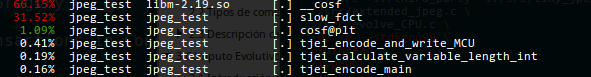
\includegraphics[width=1.0\textwidth]{pre_dct}
    \caption{Algoritmo DCT lento}
    \label{fig:pre_dct}
\end{figure}

\begin{figure}[h]
    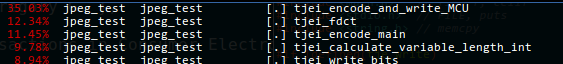
\includegraphics[width=1.0\textwidth]{post_dct}
    \caption{Algoritmo DCT rápido}
    \label{fig:post_dct}
\end{figure}


% ============================================================
\section{Micro-Optimización} \label{sec:microopt}
% ============================================================


Usamos el término \emph{micro-optimización} cuando nos referimos al tipo de
optimización de desempeño en la que no cambiamos los algoritmos que utilizamos.
Utilizamos conocimiento sobre la máquina o máquinas que van a
efectuar el cómputo para hacer cambios en la manera en que se ejecuta nuestro
algoritmo con el objetivo de obtener un mejor desempeño.

Un ejemplo de optimización que \emph{no} es micro-optimización es la
descripción del algoritmo DCT mostrado en \ref{sec:DCT}. En este ejemplo, se
logró tomar el cuello de botella de la implementación JPEG y reducirla a algo
mucho menos significativo mediante cambios algorítmicos.

Hacer micro-optimización no es recomendable hasta que uno esté seguro de que no
hay mejoras algorítmicas que puedan beneficiar el desempeño. La
micro-optimización casi siempre resulta en más código que es más difícil de
mantener. Sin embargo, cuando se llega al punto en donde no hay (o no se
ocurren) mejoras algorítmicas, podemos acelerar significativamente nuestro
programa con micro-optimización.

\subsection{GPU: Copiar bloques}

En la microarquitectura de un GPU, accesos a la memoria global usualmente
resultan en que la memoria sea copiada automáticamente a memoria local, de la
misma manera que se utilizan cachés en CPU para lidiar con la latencia de la
memoria principal. Sin embargo, no siempre podemos contar con que esto va a
suceder.

Cuando se sabe que un work item va a trabajar con un trozo de memoria de cierto
tamaño, ocasionalmente es buena idea forzar una copia a memoria local para
reducir el tiempo que el work item está esperando a memoria principal. El
siguiente pseudocódigo es una optimización común en OpenCL.

\label{alg:gpgpu-memcpy}
\begin{code}[language=C][h]
    // 64 es un número arbitrario.
    // Hay que tomar en cuenta el tamaño de la memoria local.
    int mi_copia[64];
    for (int i = 0; i < 64; ++i) {
        mi_copia[i] = memoria_global[i];
    }
\end{code}

En el caso de nuestro kernel, esta optimización resulta efectiva cuando
copiamos el \gls{MCU} (512 bytes). En la tabla \ref{fig:gpucopy} se compara el tiempo
total de nuestro programa, con tres imágenes de prueba, haciendo una copia
local vs memoria global.

\begin{figure}[h]
    \begin{tabular}{ |l c c r| }
        \hline
        Imagen & Memoria local & Memoria global & \emph{speedup} \\
        \hline
        Klay & 3.85 & 4.5 & 1.168 \\
        Diego & 1.18 & 1.44 & 1.22 \\
        Plutón & 40.16 & 47.58 & 1.1847 \\
        \hline
    \end{tabular}
    \caption{Comparación de desempeño para copia local de bloques}
    \label{fig:gpucopy}
\end{figure}

Logramos una mejora de entre 16\% y 22\% haciendo lo que a primera vista parece
más trabajo. Cabe notar que no se logra la misma mejora copiando otros
parámetros de entrada, como las tablas Huffman. Es posible que se obtiene este
desempeño adicional porque se está cargando a memoria local \emph{toda} la
memoria del bloque que va a accesarse por ese work item, mientras que el acceso
a las tablas de Huffman es mucho más aleatorio y son arreglos mucho más
grandes.

\subsection{GPU: Saltos condicionales}

Un \emph{ salto condicional } es en lo que se convierte un \verb+if+ cuando
se compila a código máquina. Para observar por qué los saltos condicionales
(usualmente llamados \emph{branches} para ahorrar teclas) son un problema en
GPU, vale la pena hacer un ejemplo.

Supóngase que un wavefront ejecuta el siguiente código:

\begin{code}[language=C][h]
    if (mi_variable) {
        funcion_a();
    } else {
        funcion_b();
    }
    funcion_c();
\end{code}

También supóngase que \verb+mi_variable+ es \verb+true+ para el 90\% de los work
items.  Cuando se llega al \verb+if+, 90\% de los work items van a ejecutar
\verb+funcion_a+, mientras que el 10\% restante va a ejecutar \verb+funcion_b+.
El problema está en que no se puede ejecutar \verb+funcion_c+ hasta que todos
los work items en el wavefront hayan terminado de ejecutar el bloque if. Esto
quiere decir que si \verb+funcion_b+ es muy cara, el 90\% del wavefront va a
estar sin hacer trabajo, esperando a que el 10\% restante termine de ejecutar
\verb+function_b+.

El kernel de DummyJPEG no puede hacer mucho para evitar que haya wavefronts
esperando saltos condicionales. Esto es por la naturaleza del algoritmo JPEG.
El procesamiento de un bloque requiere contar el número de coeficientes que son
cero, y para hacer esto es necesario iterar por todo el bloque. Encima de esto,
cada bloque tiene una cantidad de trabajo proporcional al número de
coeficientes que no son cero. Esto implica que cualquier wavefront de DummyJPEG
va a esperar al work item que tenga el menor número de ceros que procesar y por
lo tanto más trabajo que hacer.

Estar conscientes de que la palabra \verb+if+ puede ser la parte más costosa
del programa es una de las diferencias más claras cuando se hace programación
\gls{GPGPU}.


\subsection{CPU: I/O} \label{sub:cpu-io}

TinyJPEG mantiene un \emph{buffer} de 1024 bytes que se usa para minimizar
llamadas a fwrite. Las implementaciones de fwrite tratan de evitar llamadas a
sistema, pero de cualquier manera, el uso de este buffer reduce dramáticamente
el costo de escritura.

La imagen \ref{fig:fwrite} muestra el costo de fwrite en TinyJPEG con buffering
deshabilitado.

\begin{figure}[hb]
    
\includegraphics[width=5.16666in]{fputc}
    \caption{El costo de fwrite sin buffering}
    \label{fig:fwrite}
\end{figure}

Este reporte de la herramienta \verb+perf+, parte de Linux Perf Tools
\cite{linux-perf-tools}, es de un programa de prueba que carga una imagen de
Plutón de 192 MB y la codifica con TinyJPEG. Lo que se muestra es que hay dos
funciones de TinyJPEG consumiendo el 48.2\% del tiempo. También muestra que la
función \verb+fputc+ consume 4.8\% del tiempo total. Con esto concluímos que si
solo tomamos en cuenta el tiempo que se pasa codificando la imagen, se está
gastando el 9.1\% del tiempo llamando a fwrite, (que a su vez llama a putc).

No se incluye un reporte de TinyJPEG con \emph{buffering} porque al usar un
buffer de 1024 bytes, eliminamos por completo el costo de \verb+fwrite+.

La implementación de un buffer es muy simple. Este código viene directamente de TinyJPEG:

\begin{code}[language=C][h]
    // Buffer TJE_BUFFER_SIZE in memory and flush when ready
    static size_t tjei_g_output_buffer_count;
    static uint8_t tjei_g_output_buffer[TJEI_BUFFER_SIZE];
\end{code}

La manera en que nos deshacemos del problema de fwrite es escribiendo a ese
buffer.  Cuando tjei\_g\_output\_buffer\_count es igual a TJEI\_BUFFER\_SIZE,
entonces llamamos fwrite, escribiendo los contenidos del buffer completo.

Vale la pena notar que al final de la ejecución es probable que haya datos en
el buffer que no hayan sido escritos. Por eso se hace un \emph{flush} al final
del programa, haciendo una última llamada a fwrite con los contenidos del
buffer.

\subsection{CPU: Saltos condicionales}\label{sub:cpu-branch}

Para terminar las notas de micro-optimización, se va a discutir un truco en la
implementación de TinyJPEG que trata con predicción de \emph{branches} (i.e.
saltos condicionales, o bloques \verb+if+)

Los CPU son muy buenos ejecutando \emph{branches} cuando pueden predecir su
comportamiento. Agner Fog \cite{agner} tiene muy buenos recursos para estar al
día con la manera en que los procesadores de Intel predicen branches. El
concepto es que cuando el CPU piensa que un branch va a ser ejecutado, lo
ejecuta \emph{ especulativamente } mientras la condición del salto se computa
paralelamente. Se le conoce como un \emph{branch missprediction}, que
traducimos como \emph{mis-predicción de salto} a la situación en cuando el
salto se calculó especulativamente pero la condición falló. En código de alto
desempeño como la función interna de JPEG, esto puede ser un cuello de botella.

En el caso e TinyJPEG, una vez que se utilizó un algoritmo rápido de DCT, el
cuello de botella en la función \verb+encode_MCU+ resultó ser la siguiente
línea de código:

\begin{code}[language=C][h]
fval = (fval > 0)? floorf(fval + 0.5f) : ceilf(fval - 0.5f);
\end{code}

Esta es una implementación clásica de redondeo, escrita de acuerdo a la
especificación JPEG.

Usando \verb+perf+, se puede visualizar el problema (imagen \ref{fig:mispred}):

\begin{figure}[h]
    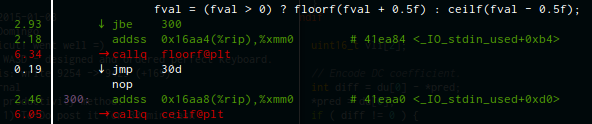
\includegraphics[width=5.16666in]{round_slow}
    \caption{Mis-predicción de salto}
    \label {fig:mispred}
\end{figure}

Ambos caminos del salto condicional inducido por el operador \verb+?:+ toman
alrededor de 9\% de los ciclos de CPU totales para esta función, con un total de 18\%.

Esa información no es suficiente para decidir que el problema es
mis-predicción, pero se puede atacar al problema como si fuera un problema de
mis-predicción. Si se hace más rápido, entonces suponemos que el problema era
el salto.

En este caso, sabemos que $fval \in [-1024, 1024]$. Esta información nos
permite evitar el salto haciendo una suma, $(fval + 1024) \in [0, 2048]$. Si
hacemos esto, podemos usar \verb+floorf+, ya que el valor siempre es positivo:

\begin{code}[language=C][h]
    fval += 1024;
    fval = floorf(fval + 0.5f);
    fval -= 1024;
\end{code}

El resultado, con \verb+perf+:

\begin{figure}[hb]
    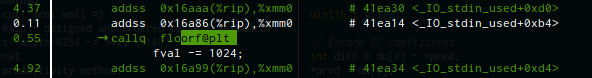
\includegraphics[width=5.16666in]{round_fast}
    \caption{Evitando mis-predicción}
\end{figure}

Como logramos alrededor de 2X de mejora en velocidad, podemos concluir con
confianza que el salto no se estaba prediciendo exitosamente, con el resultado
de que \verb+floorf+ y \verb+ceilf+ se estaban calculando \emph{siempre},
independientemente de si \verb+fval+ era positivo o negativo.



 % <- implementado! escrito! editado!

%************************************************
\chapter{Cómputo Evolutivo}\label{ch:evolucion}
%************************************************

% ============================================================
\section{Introducción a Cómputo Evolutivo}
% ============================================================

El \gls{Cómputo Evolutivo} es una rama de la Inteligencia Artificial que se define
por los tipos de algoritmos en los que se enfoca. Son algoritmos que utilizan
el concepto de la selección natural para resolver problemas de cómputo. Son
problemas de optimización en el sentido matemático. Es decir, se concentran en
encontrar un máximo local o un mínimo local utilizando heurísticas.


% ============================================================
\section{Algoritmos Evolutivos}
% ============================================================

Las características que los Algoritmos Evolutivos tienen en común son:

\begin{itemize}
\item Definen una población
\item Definen una función de selección.
\item Utilizan mutación y reproducción junto con la función de selección para
mejorar la población a lo largo de varias generaciones.
\end{itemize}

Aunque comparten la misma idea, se definen distintos tipos de algoritmos con
respecto a la manera en que concretizan estas características.

\begin{itemize}
\item La \emph{Programación Genética} \cite{GenProg} tiene conjuntos de
programas como su población. Su función de selección es la capacidad de un
programa para resolver cierto problema. Los programas se representan como
árboles de sintaxis, y de esta manera se define la mutación y reproducción como
operaciones en árboles.
\item La \emph{Programación Evolutiva} es similar a la Programación Genética
pero lo que se evoluciona son los parámetros de los programas, no su
estructura.
\item Los \emph{Algoritmos Genéticos} definen genotipos y su correspondiente
función de selección que evalúa los fenotipos respectivos. Es decir, se opera
sobre el cromosoma pero se evalúa el organismo.

El algoritmo desarrollado entra dentro de la clasificación de Algoritmo
Genético. El fenotipo es una tabla de cuantificación y el genotipo es un
codificador \gls{JPEG} que usa esa tabla.

\end{itemize}

% ============================================================
\section{Método para la evolución de codificadores JPEG}
% ============================================================

\subsection{Población}

Se inicializa una población de tablas. En el conjunto se incluye la tabla que
tiene todos sus coeficientes iguales a 1, denominada \emph{\gls{tabla
unitaria}}. La tabla unitaria es la que obtiene la mejor calidad posible pero
resulta en menor compresión. El resto del conjunto se llena de tablas con
valores aleatorios entre 1 y 64.

La función de selección requiere de un punto de referencia. Antes de iniciar la
evolución, se comprime la imagen con la tabla unitaria, dándonos un punto de
referencia para la calidad óptima y para el máximo tamaño.

\subsection{Selección}

La calidad de la compresión se determina haciendo una decodificación y
comparando la imagen resultante con la original píxel por píxel. Las
diferencias absolutas se suman. No se utiliza MSE (Error cuadrático medio) por
la enorme cantidad de pixeles y la sensibilidad del algoritmo a errores de
precisión. En lugar de implementar un decodificador JPEG, se incluye un paso de
decodificación en la función principal de procesamiento de bloques. Los
detalles de este proceso se explican en el capítulo \ref{ch:implementacion}.

El tamaño es más fácil de comparar que la calidad de la imagen. Tan solo es
necesario ver cuántos bits pesa la imagen resultante comparada con el tamaño
máximo que se obtiene de la tabla unitaria.

Tenemos dos garantías. Cualquier tabla de cuantificación comparada con la
unitaria va a resultar en mayor compresión y en menor calidad, siempre y cuando
la tabla a comparar no sea en sí una tabla unitaria.

Sea $T$ una tabla de nuestra población y sea $T_0$ la tabla unitaria.

Definimos nuestra función de selección como:

\begin{equation}
f(T) = \frac{e(T)}{e(T_0)} + \alpha \Big(1 + \frac{s(T)}{s(T_0)}\Big)
\end{equation}\label{eq:fitness}

\dots donde $e(T)$ es el error de compresión y $s(T)$ es el tamaño de la
imagen. $\alpha$ es una constante que se usa para ajustar la importancia que le
damos al tamaño sobre la compresión o vice versa.

Nótese que los dos términos se afectan mutuamente. Una tabla que tiene mayor
compresión va a tener un mayor error, y una tabla con menor compresión resulta
en una imagen de mayor calidad. En otras palabras, cuando el primer término
disminuye, el segundo crece.  Cuando el segundo término crece, el primero
disminuye.

Nuestra meta es encontrar $T$ tal que $f(T)$ es mínima. La relación entre los
dos términos permite que el algoritmo converja.

El primer término es siempre mayor o igual a $1$. A la fracción del segundo
término se le suma 1 porque el valor de $\frac{s(T)}{s(T_0)} \in (0, 1]$. Esto
es puramente una una conveniencia para facilitar la búsqueda de un valor de
$\alpha$ adecuado.

El valor de $\alpha$ controla el proceso de minimización. Mientras mayor sea
$\alpha$, más peso de selección tiene el tamaño de la imagen. El algoritmo tiende
a 'preferir' minimizar el error contra el tamaño después de cierto umbral de
$\alpha > 1$. Para valores de $alpha <= 1$, se producen imágenes de muy mala calidad.

Habiendo probado varios valores distintos, se encontró que un valor de $\alpha
= 2$ resulta en imágenes que son indistinguibles de las originales, con un alto
nivel de compresión.


\subsection {Mutación y Reproducción}

Cada generación, sobreviven las dos mejores tablas. El resto se parte en dos.

Con las pruebas que se hicieron, se encontró que con el método de cruza y de
mutación que se está utilizando, la taza más efectiva es dividir 50\% de la
población para ser mutada, y 50\% para ser cruzada. En la mayoría de los casos
esto resultó en una convergencia más rápida con mejores valores al evaluar la
función de selección.

El proceso de mutación es como sigue: Cada entrada de la tabla tiene una
probabilidad de $\frac{1}{64}$ de mutar. Cuando una entrada $e$ muta, lo hace
sumando a su valor original $e_{nueva} = e_{vieja} + x $ donde $x \in [-4, 4]$
con distribución de probabilidad uniforme.

El proceso de reproducción siempre ocurre entre las dos tablas ganadoras. Padre
A y Padre B.  La tabla hijo es el resultado de, para cada entrada, escoger una
entrada de Padre A o de Padre B. La elección es un tiro de moneda. Para alguno
de los dos padres, cada entrada tiene un $50\%$ de probabilidad de venir de él.

\subsection {Fin de la evolución}

El algoritmo decide terminar cuando sucede una de dos cosas:

\begin{itemize}
\item El número de generaciones llega a 100
\item La diferencia entre el valor de la función \ref{eq:fitness} para el
individuo más apto es menor a 0.0001 cuatro veces consecutivas. En este caso,
se decide que la evolución ha convergido.
\end{itemize}

Al final de la evolución, se toma la tabla ganadora y se usa como entrada para
el codificador \gls{JPEG}.

 % <- RE-ESCRIBIR, RE-IMPLEMENTAR, RE-EDITAR

%************************************************
\chapter{Conclusiones}\label{ch:conclusiones}
%************************************************

El proyecto presentado en esta tesis aprovecha los saltos tecnológicos que se
han dado desde la creación de JPEG en 1992 \cite{jpeg-spec} para lograr mejor
resultados usando un formato ya existente. El algoritmo produce buenos
resultados consistentemente, y ocasionalmente consigue simultáneamente una
mejor calidad de imagen y una mayor compresión.

Se hizo mención en un par de ocasiones a que el programa está diseñado para
producir imágenes \emph{indistinguibles} de las originales, sin mencionar el
hecho de que es imposible medir las características cualitativas del sistema
visual humano. Se utilizó una métrica estándar de diferencia \emph{pixel por
pixel} para determinar el error de imagen, pero esta no es la única opción
disponible. Existe un área de investigación dedicada a medir la calidad de
imágenes tomando en cuenta modelos basados en el sistema visual humano
\cite{subjective-paper}.

% Nuevos formatos (Mr. Bellard) que pretenden reemplazar a JPEG.
Recientemente ha habido esfuerzos para reemplazar a JPEG en la web,
notablemente por Google (\cite{brotli}, \cite{webp}). El mayor problema a
resolver es el de inercia. Google usa su poder sobre el Internet, pero esta no
es la única estrategia. Francis Bellard, creador de Qemu, FFmpeg y otros
proyectos de código libre, lanzó un formato llamado \gls{BPG}, cuyo
decodificador está escrito en Javascript, y por lo tanto tiene una adopción
virtualmente universal.

Sin embargo, JPEG no se va a ir a ningún lado. Usar la fuerza bruta de las
máquinas comunes de hoy en día también es una buena estrategia para obtener una
mejora sobre un formato que ya está en la médula del mundo del software.

% Distribución de programas que usan OpenCL
Se utilizó OpenCL para la paralelización en GPUs por ser un formato abierto y
por que actualmente está adoptado por todos los proveedores de cómputo
vectorial masivo (Intel, NVidia y AMD). Actualmente es difícil distribuir de
manera binaria un codificador que use OpenCL. Se tiene la esperanza de que en
el futuro exista una manera inmediata de utilizar las capacidades de cómputo
vectorial que son cada vez más ubicuas.

En las últimas dos décadas ha habido una tendencia hacia una convergencia entre
GPU y CPU. Aunque hoy en día se tiene que escribir código en lenguajes
propietarios o con herramientas primitivas, es claro hacia donde se está
moviendo la marea. Por el lado del hardware, Intel y Nvidia están dando
soluciones para cómputo de alto desempeño con sus productos Xeon Phi y Tesla,
respectivamente. En el lado del consumidor, los procesadores de escritorio de
Intel dedican una porción cada vez más grande de los transistores disponibles a
una unidad de gráficas integradas, que hoy en día puede ser aprovechada con
OpenCL. Los GPUs, por otro lado están, generación tras generación, volviéndose
más programables. Cada día hay más información disponible para el programador
que quiera usar el poder de los GPUs.

Este proyecto aprovechó el hecho de que JPEG cuenta con un problema para el
cual no existe solución, y fue exitoso en lograr su propósito mediante el uso
de \gls{Cómputo Evolutivo}. Los algoritmos genéticos fueron una gran herramienta
para conseguir una solución heurística al problema de las tablas de
cuantificación.

Los algoritmos genéticos se prestan a ser programados con \gls{GPGPU}. La
necesidad de alto rendimiento y la tendencia a que no importe tener alta
latencia sugieren que los GPUs pueden ser usados. Si la función de selección es
una función pura y el problema es demandante, entonces no hay razón para no
hacer una implementación en el GPU.
 % escrito! editado!

\chapter{Apéndice}\label{ch:apendice}

\section{Glosario}


\end{document}

%%% Local Variables:
%%% mode: latex
%%% TeX-engine: xetex
%%% TeX-master: t
%%% End:
